\chapter{Diodes lasers à semi-conducteurs}
\section{Propriétés électroniques des semi-conducteurs}
	\subsection{Modèle de l'électron libre}
	Il s'agit du modèle le plus simple pour décrire les propriétés des électrons libre dans 
	un cristal : on suppose que l'électron est totalement libre et de fonction d'onde dépendante
	du temps
	\begin{equation}
	\psi ({\bf{r}},t) = \varphi ({\bf{r}}){{\rm{e}}^{ - i\frac{{\rm{E}}}{\hbar }t}}
	\end{equation}
	En une dimension
	\begin{equation}
	- \frac{{{\hbar ^2}}}{{2{m_e}}}\frac{{{{\rm{d}}^2}}}{{{\rm{d}}{x^2}}} + \underbrace{V(x)}_{=0}]
	\varphi (x) = {\rm{E}}	\varphi (x)
	\end{equation}
	Les solutions sont données par
	\begin{equation}
	\varphi (x) = \exp (ikx)\qquad\Rightarrow\qquad {\rm{E}} = \frac{{{\hbar ^2}{k^2}}}{{2{m_e}}}
	\end{equation}
	\begin{wrapfigure}[11]{l}{6cm}
	\vspace{-5mm}
	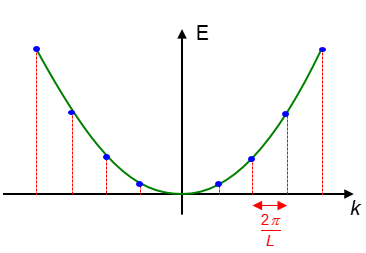
\includegraphics[scale=0.6]{ch5/image1}
	\captionof{figure}{ }
	\end{wrapfigure}

	Il s'agit bien d'une onde plane. En appliquant à celle-ci les conditions de BVK (périodicité 
	multiple de constante de réseau $a$, $\varphi(x+L) = \varphi(x)$), il faut que $k$ soit un 
	multiple entier de $2\pi$
	\begin{equation}
	k = p\frac{2\pi}{L}\qquad k\in\mathbb{Z}
	\end{equation}
	Seules des valeurs discrètes de l'énergie sont autorisées et on en tire une relation de 
	dispersion parabolique $E=f(k)$.\\
	
	En généralisant à 3D avec le vecteur d'onde ${k^2} = k_x^2 + k_y^2 + k_z^2$
	\begin{equation}
	{k_x} = p\frac{{2\pi }}{L};{\rm{  }}{k_y} = q\frac{{2\pi }}{L};{\rm{  }}{k_z} = r\frac{{2\pi }}{L}
	\end{equation}
	Par facilité, on va regarder ce qui se passe dans l'espace réciproque composé de cellules 
	cubiques élémentaires. Les électrons essayent de minimiser leur énergie et donc leur $k_i$ 
	dans l'espace réciproque. Ce sont des fermions : il ne peut pas y avoir $k_x=k_y=k_z=0$ et 
	ils vont donc remplir l'espace réciproque comme une sphère\footnote{$k_F$ correspond au 
	niveau d'énergie maximal à température nulle.}. A $T=0K : k\leq k_F$ (sphère).
	L'énergie de Fermi dans un cristal libre est donné par
	\begin{equation}
	{{\rm{E}}_F} = \frac{{{\hbar ^2}k_F^2}}{{2{m_e}}}
	\end{equation}
	Que vaut $E_F$ ? Le nombre d'électron dans un cristal est donné par ${N_e} = {n_e}{L^3}$ soit 
	encore
	\begin{equation}
	{N_e} = 2.\frac{{{4 \mathord{\left/
	 {\vphantom {4 3}} \right.
	 \kern-\nulldelimiterspace} 3}\pi k_F^3}}{{{{(2\pi /L)}^3}}}
	\end{equation}
	\begin{wrapfigure}[9]{l}{4cm}
	\vspace{-5mm}
	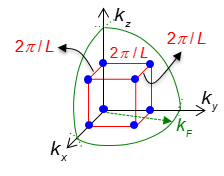
\includegraphics[scale=0.6]{ch5/image2}
	\captionof{figure}{ }
	\end{wrapfigure}
	où le facteur deux corresponds aux états possibles par point dans l'espace $k$ (deux spins). 
	On multiplie ensuite par le volume de la sphère de Fermi et on divise par le volume d'une 
	maille élémentaire. On en tire
	\begin{equation}
	{k_F} = {[3{\pi ^2}{n_e}]^{1/3}}\qquad\Rightarrow\qquad {{\rm{E}}_F} = {\hbar ^2}{[3{\pi ^2}{n_e}]^{2/3}}/(2{m_e})
	\end{equation}	
	C'est bien indépendant de la maille du cristal et c'est pour ça qu'on a pris un cube. 
	
	
	\subsection{Modèle de l'électron quasi-libre}	
	On suppose dans ce modèle qu'il y a des interactions faibles avec les ions du cristal 
	donnant lieu à une probabilité non nulle de réflexion (mais très faible) de la fonction 
	d'onde
	\begin{equation}
	r^2+t^2 = 1,\qquad r\ll 1
	\end{equation}
	Dans un cas 1D, l'électron incident peut être réfléchi partiellement sur chacun des 
	atomes du cristal
	\begin{equation}
	R = r{{\rm{e}}^{ik2a}} + {t^2}r{{\rm{e}}^{ik4a}} + {t^4}r{{\rm{e}}^{ik6a}} + ... =
	r{{\rm{e}}^{ik2a}}(1 + {t^2}{{\rm{e}}^{ik2a}} + {t^4}{{\rm{e}}^{ik4a}} + ...)
	\end{equation}
	\begin{center}
	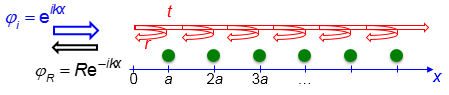
\includegraphics[scale=0.7]{ch5/image3}
	\captionof{figure}{ }
	\end{center}
	Il s'agit d'une suite géométrique 
	\begin{equation}
	R = \frac{{r{{\rm{e}}^{ik2a}}}}{{1 - {t^2}{{\rm{e}}^{ik2a}}}}
	\end{equation}
	où $|t|^2 <1$. Si le terme de phase vaut 1 alors $R=1$
	\begin{equation}
	R = 1\qquad\Leftrightarrow\qquad ka=m\pi
	\end{equation}
	Même si les probabilités sont très faible, l'électron sera réfléchi à un moment.\\
	
	Pour tirer quelques conclusions intéressantes, résolvons l'ED de Schrödinger 1D à la 
	résonance
	\begin{equation}
	[ - \frac{{{\hbar ^2}}}{{2{m_e}}}\frac{{{{\rm{d}}^2}}}{{{\rm{d}}{x^2}}} + V(x)]\varphi (x) = {\rm{E}}\varphi (x)
	\end{equation}
	où $V(x)$ est le potentiel d'interaction. Nous allons chercher une solution sous la forme 
	d'une onde incidente et une réfléchie, le but étant de déterminer $R$ en fonction de $k$ 
	pour en déduire l'énergie.
	\begin{equation}
	\varphi (x) = \exp (ikx) + R\exp ( - ikx)
	\end{equation}


	\begin{wrapfigure}[7]{r}{4cm}
	\vspace{-5mm}
	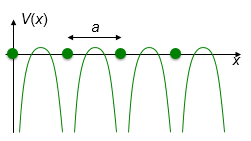
\includegraphics[scale=0.6]{ch5/image4}
	\captionof{figure}{ }
	\end{wrapfigure}
	Développons en série le potentiel
	\begin{equation}
	V(x) =  - {V_1}\cos (2\pi x/a) + {V_2}\cos (4\pi x/a) + ...
	\end{equation}
	L'interaction étant faible, nous ne gardons que le premier ordre. Il en vient alors
	\begin{equation}
	\left[ {\frac{{{\hbar ^2}{k^2}}}{{2{m_e}}} - \frac{{{V_1}}}{2}({{\mathop{\rm e}\nolimits} ^{i2\pi x/a}} + {{\mathop{\rm e}\nolimits} ^{ - i2\pi x/a}})} \right]({{\mathop{\rm e}\nolimits} ^{ikx}} + R{{\mathop{\rm e}\nolimits} ^{ - ikx}}) = {\rm{E}}({{\mathop{\rm e}\nolimits} ^{ikx}} + R{{\mathop{\rm e}\nolimits} ^{ - ikx}})
	\end{equation}
	Multiplions par $e^{\pm ikx}$ et intégrons
	\begin{equation}
	\left\{\begin{array}{llll}
	\DS \frac{1}{L}\int\limits_{ - L/2}^{L/2} {... \times {{\mathop{\rm e}\nolimits} ^{ - ikx}}{\rm{d}}x} &\DS\quad\Rightarrow\quad \frac{{{\hbar ^2}{k^2}}}{{2{m_e}}} - \frac{{{V_1}}}{{2L}}R\int\limits_{ - L/2}^{L/2} {\exp [i2(\frac{\pi }{a} - k)x]{\rm{d}}x}  &\DS= {\rm{E}}&\qquad(1)\\
	\DS\frac{1}{L}\int\limits_{ - L/2}^{L/2} {... \times {{\mathop{\rm e}\nolimits} ^{ikx}}{\rm{d}}x}&
	\DS\quad\Rightarrow\quad \frac{{{\hbar ^2}{k^2}}}{{2{m_e}}}R - \frac{{{V_1}}}{{2L}}\int\limits_{ - L/2}^{L/2} {\exp [ - i2(\frac{\pi }{a} - k)x]{\rm{d}}x}  &\DS= {\rm{E}}R&\qquad(2)
	\end{array}\right.
	\end{equation}
	Si l'on est loin de la condition de réflexion de Bragg ($k\neq \pi/a$) on retrouve la même 
	relation de dispersion que pour un électron libre
	\begin{equation}
	\int\limits_{ - L/2}^{L/2} {...{\rm{d}}x}  \approx 0\qquad\Rightarrow\qquad E = \frac{{{\hbar ^2}
	{k^2}}}{{2{m_e}}}
	\end{equation}
	A la réflexion de Bragg, nous avons des interférences constructrices avec l'onde réfléchie.
	En effectuant $(1).R-(2)$, on trouve pour $R=1$
	\begin{equation}
	{\rm{E}} = \frac{{{\hbar ^2}{k^2}}}{{2{m_e}}} - \frac{{{V_1}}}{2}\quad \Rightarrow\quad
	|\varphi {\rm{(x)}}{{\rm{|}}^{\rm{2}}} \propto 1 + {\rm{cos(2}}\pi x/a{\rm{)}}
	\end{equation}
	Il s'agit de l'énergie de l'électron libre diminuée d'un petit quelque-chose. Pour $R=-1$
	\begin{equation}
	{\rm{E}} = \frac{{{\hbar ^2}{k^2}}}{{2{m_e}}} + \frac{{{V_1}}}{2}\quad\Rightarrow\quad
	{\rm{ }}|\varphi {\rm{(x)}}{{\rm{|}}^{\rm{2}}} \propto {\rm{1 - cos(2}}\pi x/a{\rm{)}}
	\end{equation}
	\begin{center}
	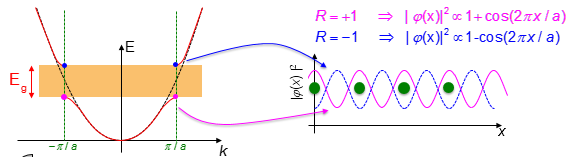
\includegraphics[scale=0.76]{ch5/image5}
	\captionof{figure}{ }
	\end{center}
	Si on trace en fonction de $x$,le maximum de probabilité coïncide avec la position de l'atome 
	et on peut interpréter ça comme un électron lié à l'atome et l'énergie est logiquement plus 
	faible. Dans l'autre cas, il est "entre" les atomes et donc libre de se mouvoir.\\
	
	\begin{wrapfigure}[9]{r}{3.5cm}
	%\vspace{-5mm}
	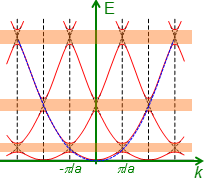
\includegraphics[scale=0.6]{ch5/image6}
	\captionof{figure}{ }
	\end{wrapfigure}
	L'approche plus rigoureuse du formalisme s'obtient avec les modes de Bloch qui ont la périodicité
	du cristal
	\begin{equation}
	\varphi ({\bf{r}}) = {u_k}({\bf{r}})\exp (i{\bf{k}}.{\bf{r}})
	\end{equation}
	Elles impliquent une relation de dispersion périodique dans l'espace $\vec k$, de période 
	$2\pi/a$. Cette périodicité fait part à une structure en bandes permises et interdites. Afin 
	de savoir quelles bandes sont remplies, il est nécessaire de connaître la capacité d'une bande.
	Si l'on regarde dans l'espace $\vec k$ on retrouve la longueur totale divisée par l'écart entre
	deux niveaux, le tout multiplié par 2 pour tenir compte du spin
	\begin{equation}
	{N_{{\rm{states}}}} = 2.\frac{{[2\pi /a]}}{{[2\pi /L]}} = 2\frac{L}{a}{\rm{ }} = \text{2*
	nombre d'atomes}
	\end{equation}
	où $L/a$ est le nombre d'atomes. Dès lors, le nombre d'électron disponible est donné par la 
	valence multipliée par le nombre d'atomes\footnote{Exemples slide 7.}.\\
	
	A température nulle, il n'y a que des bandes complètement remplies : la dernière est la bande
	de valence et la première vide est la bande de conduction. On appelle l'\textit{énergie du gap}
	$E_g$ l'énergie entre la bande de valence et la bande de conduction. Avoir des bandes remplies 
	ou non influe sur les propriétés électroniques
	\begin{itemize}
	\item[$\bullet$] $E=0$ : les électrons se distribuent symétriquement autour de $\vec{k}=\vec 0
	\to \langle\vec{k}\rangle = 0\to \langle \vec v\rangle=0$ et ce même si il existe des électrons
	avec $\vec{k}\neq\vec{0}$.
	\item[$\bullet$] Si la bande est pleine, les électrons ne peuvent pas bouger et on a les même 
	conclusions que pour le cas $E=0$. Si la bande est partiellement remplie les électrons vont 
	bouger : asymétrie et vitesse moyenne non nulle $\to$ densité de courant non nulle, c'est un 
	conducteur (Na, Li, \dots) !
	\end{itemize}
	\begin{center}
		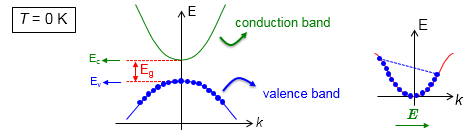
\includegraphics[scale=0.8]{ch5/image7}
	\captionof{figure}{ }
	\end{center}
	
	\begin{wrapfigure}[9]{l}{3.5cm}
	\vspace{-5mm}
	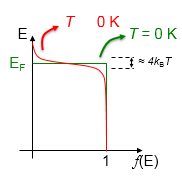
\includegraphics[scale=0.6]{ch5/image8}
	\captionof{figure}{ }
	\end{wrapfigure}
	Imaginons une bande partiellement remplie. A température nulle, tous les états sont occupés
	jusqu'à $k=k_F \to E\leq E_F$. Si la température n'est pas nulle, à l'équilibre thermique, la
	probabilité d'occupation d'un niveau d'énergie $E$ est donné par la distribution de Fermi-Dirac
	\begin{equation}
	f({\rm{E}}) = \frac{1}{{1 + \exp [({\rm{E}} - {{\rm{E}}_{\rm{F}}})/{k_{\rm{B}}}T]}}
	\end{equation}
	Si la dernière bande est remplie, c'est un peu différent : dans l'espace $\vec k$ on a toujours
	un empilement jusque $k=k_F$ mais le nombre d'états occupé est donné par
	\begin{equation}
	\text{valence}*\frac{L}{a} = 2.\frac{{2{k_F}}}{{(2\pi /L)}}\quad\Rightarrow\quad
	{k_F} = \frac{{{\rm{valence}}}}{2}\frac{\pi }{a}
	\end{equation}
	
	\begin{wrapfigure}[9]{r}{3.5cm}
	\vspace{-5mm}
	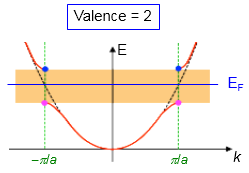
\includegraphics[scale=0.6]{ch5/image9}
	\captionof{figure}{ }
	\end{wrapfigure}
	On a $2k_F$ qui s'empilent dans l'espace $\vec k$ jusque $k_F$ mais dans $[-k_F,+k_F]$ on 
	divise par la longueur. Pour les atomes avec une valence paire,$k_F$ est sur le bord de la 
	zone de Brillouin. On en tire l'énergie de Fermi qui se situe au \textbf{milieu} de la bande
	interdite\footnote{\danger\ Elle ne vaut pas l'énergie maximale $E_v$ pour $T=0K$.}
	\begin{equation}
	E_F = \dfrac{\hbar^2k_F^2}{2m_e}
	\end{equation}
	Dans le cas où $T\neq 0K$, si $E_g\gg1$ il s'agit d'un isolant et si $E_g\leq 1$, un 
	semi-conducteur (la conductivité augmente avec $T$). Si on applique un champ électrique 
	$E$ en présence d'un défaut d'électron, ceux-ci vont migré (voir schéma) vers la gauche 
	tandis que les trous dans le sens d'application du champ. Le défaut d'électron peut être
	vu comme une charge $+e$ se déplaçant vers la droite. Plutôt que de regarder les électrons, 
	on peut adopter une vision équivalente qui consiste à regarder les trous.
	\begin{center}
	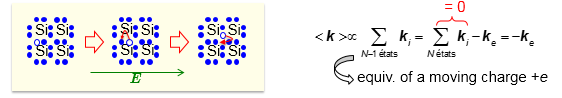
\includegraphics[scale=0.6]{ch5/image10}
	\captionof{figure}{Une absence d'électron dans la bande de valence est un \textit{trou}}
	\end{center}
	Les électrons essayent de minimiser leurs énergie : ils vont descendre et les trous monter. On 
	localise ainsi les $e^-$ près du minimum de la bande de conduction d'énergie $E_c$ et les trous
	près du maximum de la bande de valence d'énergie $E_v$. Les propriétés électroniques et 
	optiques dépendent ainsi des charges libres près des extréma des bandes de valence et conductions.\\

	Pour tenir compte des effets de répulsions des $e^-$ causée par $E$, on travaille généralement
	avec une approche semi-classique : la \textit{masse effective}. Sachant que 
	\begin{equation}
	F = qE = \hbar\frac{d}{dt}k\quad\Rightarrow\quad v_g = \frac{{{\rm{d}}\omega }}{{{\rm{d}}k}} =
	\frac{1}{\hbar }\frac{{{\rm{dE}}}}{{{\rm{d}}k}}
	\end{equation}
	On peut en tirer l'accélération et déduire la masse effective
	\begin{equation}
	\frac{{\rm{d}}}{{{\rm{d}}t}}{v_g} = \frac{{{\rm{dk}}}}{{{\rm{d}}t}}\frac{{\rm{d}}}{{{\rm{d}}k}}{v_g} = \frac{1}{\hbar }\frac{{{\rm{dk}}}}{{{\rm{d}}t}}\frac{{{{\rm{d}}^2}{\rm{E}}}}{{{\rm{d}}{k^2}}}
	\qquad\Rightarrow\qquad {m_{eff}} = F/acc. = \frac{{{\hbar ^2}}}{{{{\rm{d}}^2}{\rm{E/d}}{k^2}}}
	\end{equation}
	
	Pour un traitement plus simple, nous allons faire l'approche parabolique consistant à approcher 
	la relation de dispersion aux extréma de bande comme une parabole. En supposant $m_{eff}=c^{te}$
	\begin{description}
	\item[Bande de conduction] ${\rm{E}} = {{\rm{E}}_c} + \frac{{{\hbar ^2}{k^2}}}{{2{m_c}}}$
	\item[Bande de valence] ${\rm{E}} = {{\rm{E}}_v} - \frac{{{\hbar ^2}{k^2}}}{{2{m_v}}}$
	\end{description}
	Le comportement des $e^-$/trous est très proche du comportement d'une charge libre : on va 
	remplacer la vraie masse de l'électron/trou par $m_c/m_v$ pour modéliser leurs interactions.
	
	
	\subsection{Densité électronique d'états $\rho_e$}	
	On la défini telle que $\rho_e(E)\text{d}E$ est le nombre d'état électronique qui ont une 
	énergie entre $E$ et $E+\text{d}E$ par unité de volume. Nous allons voir que si un côté du 
	cristal est très petit les propriétés seront modifiées mais pour l'instant considérons un 
	petit cube de longueur $L$. Calculons la densité (exprimée en énergie) en fonction de $k$ (
	simple car empilement dans l'espace des états)
	\begin{equation}
	{\rho _e}(k){\rm{d}}k = \frac{1}{V}2\frac{{4\pi {k^2}{\rm{d}}k}}{{{{(2\pi /L)}^3}}} = \frac{{{k^2}{\rm{d}}k}}{{{\pi ^2}}}
	\end{equation}
	On calcule ici le nombre d'états qui ont un nombre d'onde entre $k$ et $k+dk$. Dans l'espace 
	$k$, le volume de la calotte sphérique vaut $4\pi k^2dk$, on divise par le volume occupé par 
	chaque électron $(2\pi/L)^3$, on divise encore par le volume comme on veut par volume et on 
	multiplie par 2 pour tenir compte du spin. Le résultat ci-dessus après simplification est très
	proche du résultat que nous avions pour les photons lors du calcul de la densité spectrale de 
	mode. Faisons varier l'énergie : ${\rm{dE}} = \frac{{{\hbar ^2}k}}{{{m_e}}}{\rm{d}}k$. Dès lors
	\begin{equation}
	\frac{{{k^2}}}{{{\pi ^2}}}{\rm{d}}k = \frac{{{k^2}}}{{{\pi ^2}}}\frac{{{m_e}}}{{{\hbar ^2}k}}{\rm{dE}}\quad\Rightarrow\quad {\rho _e}({\rm{E}}){\rm{dE}} = \frac{1}{{2{\pi ^2}}}{\left( {\frac{{2{m_e}}}{{{\hbar ^2}}}} \right)^{3/2}}\sqrt {\rm{E}} {\rm{dE}}
	\end{equation}
	On retrouve une variation en $\sqrt{E}$ typique du cristal 3D. Si on tient compte que les 
	porteurs de charges ne sont pas libre et qu'ils sont en particulier dans la bande de valence 
	ou de conduction\footnote{Pour la conduction $E=E_c+\dots$}, on en tire les \textbf{densité 
	d'états dans les bandes de conductions et de valences}
	\begin{description}
	\item[Bande de conduction] $\DS {\rho _c}({\rm{E}}) = \frac{{{{(2{m_c}/{\hbar ^2})}^{3/2}}}}
	{{2{\pi ^2}}}\sqrt {{\rm{E - }}{{\rm{E}}_c}} ,{\rm{     \qquad( E  >  }}{{\rm{E}}_c})$
	\item[Bande de valence]	$\DS {\rho _v}({\rm{E}}) = \frac{{{{(2{m_v}/{\hbar ^2})}^{3/2}}}}{{2{\pi ^2}}}\sqrt {{{\rm{E}}_v}{\rm{ - E}}} ,{\rm{    \qquad ( E  <  }}{{\rm{E}}_v})$
	\end{description}
	
	
	\subsection{Probabilité d'occupation et densité de porteurs}
		\subsubsection{Densité de porteurs à l'équilibre thermique}
		Pour un semi-conducteur à l'équilibre, deux cas :
		\begin{enumerate}
		\item Le nombre d'électron par unité d'énergie dans la bande de conduction : $\rho_c(E)f(E)$
		\item Le nombre de trous par unité d'énergie dans la bande de valence : $\rho_c(E)[1-f(E)]$		
		\end{enumerate}
		où $[1-f(E)]$ est la probabilité de ne pas avoir d'électrons. Pour avoir la densité dans la 
		bande de conduction, il suffit d'intégrer
		\begin{equation}
		{n_e} = \int_{{E_c}}^\infty  {{\rho _c}({\rm{E}})f({\rm{E}}){\rm{dE}}} 
		\end{equation}
			\begin{center}
	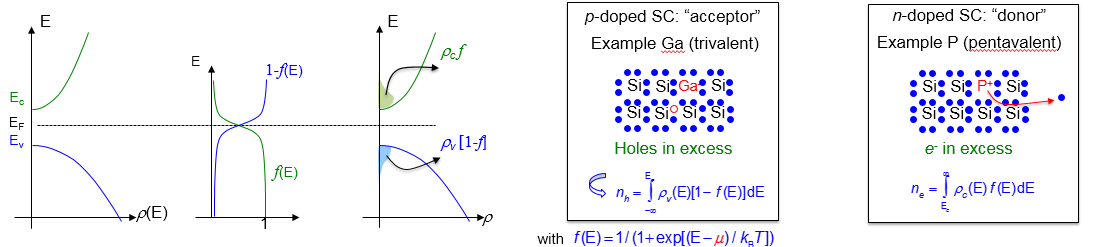
\includegraphics[scale=0.5]{ch5/image11}
	\captionof{figure}{ }
	\end{center}
	
	\begin{wrapfigure}[4]{l}{6cm}
	\vspace{-5mm}
	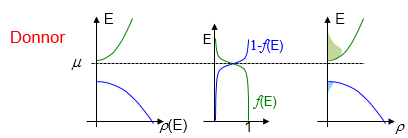
\includegraphics[scale=0.5]{ch5/image12}
	\captionof{figure}{ }
	\end{wrapfigure}
	Si on dope $n$ il y aura plus d'électron et quelque chose doit changer. Ce quelque chose est
	forcément la distribution : on ne va plus considérer l'énergie de Fermi mais le potentiel 
	chimique $\mu$.
\newpage	
	\subsubsection{Densité de porteurs en dehors de l'équilibre thermique}
		\begin{wrapfigure}[6]{r}{6cm}
	\vspace{-5mm}
	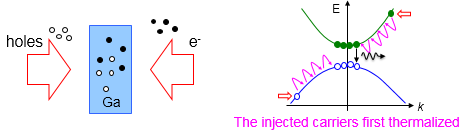
\includegraphics[scale=0.5]{ch5/image13}
	\captionof{figure}{ }
	\end{wrapfigure}
	Lorsque l'on génère un électron libre, on génère un trou dont la densité est donnée par celle
	de Fermi. Il est possible d'injecter des charges mobiles dans le milieu : d'un côté les 
	électrons et de l'autre les trous. Ces porteurs injectés vont d'abord thermaliser (0.1 ps) 
	pour ensuite se recombiner (1 ns), soit le temps de vie dans la bande de valence. Lors de la
	recombinaison des électrons avec un trou, ils vont redescendre dans la bande de valence. On dit 
	que les porteurs sont rapidement dan un état de \textit{quasi-équilibre thermique}.\\
	
	Ainsi, la densité de porteurs $\rho$ ne change pas par rapport à l'équilibre thermique lors de
	l'ajout de charges\footnote{Pq ?} mais il y a par contre une modification de la probabilité
	d'occupation dans les bandes de valences et conductions.\ \\
	
	\cadre{
	\begin{equation}
	{n_e} = \int\limits_{{{\rm{E}}_c}}^\infty  {{\rho _c}({\rm{E}}){f_c}({\rm{E}}){\rm{dE}}} \quad
	\text{ avec}\quad {f_c}({\rm{E}}) = {\left( {1 + \exp [({\rm{E}} - {{\rm{E}}_{fc}})/{k_{\rm{B}}}T]} \right)^{ - 1}}
	\end{equation}
	\begin{equation}
	{n_t} = \int\limits_{ - \infty }^{{{\rm{E}}_v}} {{\rho _v}({\rm{E}})[1 - {f_v}({\rm{E}})]
	{\rm{dE}}} \quad\text{ avec } {f_v}({\rm{E}}) = {\left( {1 + \exp [({\rm{E}} - {{\rm{E}}_{fv}})
	/{k_{\rm{B}}}T]} \right)^{ - 1}}
	\end{equation}}\ \\	

	\begin{wrapfigure}[10]{l}{6cm}
	\vspace{-5mm}
	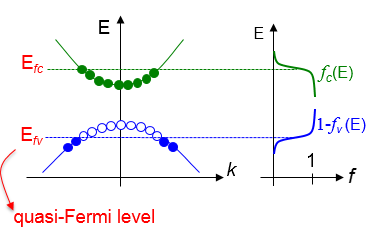
\includegraphics[scale=0.5]{ch5/image14}
	\captionof{figure}{ }
	\end{wrapfigure}
	Nous avons ainsi utilisé, respectivement pour les électrons et les trous
	\begin{equation}
	f(E)\Rightarrow f_c(E),\qquad\qquad 1-f(E) = 1-f_v(E)
	\end{equation}
	La différence entre $f_c$ et $f_v$ donne la valeur de la \textbf{quasi énergie de Fermi} dans 
	la bande de conduction ($E_{fc}$) et de valence ($E_{fv}$). Ces quasi énergies sont dépendantes 
	de la densité d'électrons ($n_e$) et de trous ($n_t$) à l'équilibre thermique.\ \\
	
	\textsc{Application : jonction pn}\\
	Considérons une zone dopée $n$ et une autre dopée $p$. En les mettant en contact, un potentiel
	$-e\Delta\varphi$ est présent à cause de la zone de charge d'espace.
	\begin{center}
	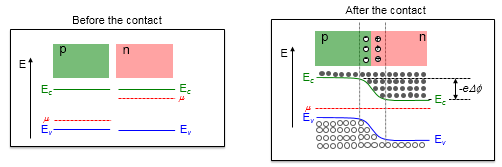
\includegraphics[scale=0.75]{ch5/image15}
	\captionof{figure}{ }	
	\end{center}
	\newpage
	\begin{wrapfigure}[8]{r}{4.5cm}
	\vspace{-5mm}
	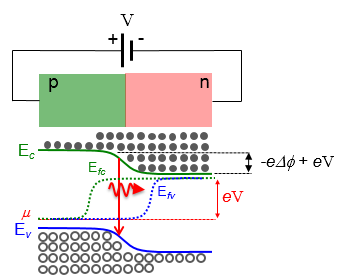
\includegraphics[scale=0.5]{ch5/image16}
	\captionof{figure}{ }
	\end{wrapfigure}
	L'application d'une tension va se ressentir dans la région de charge d'espace, les charges étant
	mobiles. En appliquant une tension positive en $V$ cela diminue la différence de potentiel et on 
	va avoir migrations des électrons de $p$ vers les trous de $n$ : la densité d'électrons-trous 
	augmente dans la région centrale et on s'attend à une recombinaison. On peut ainsi voir une 
	évolution des quasi niveaux de Fermi avec la position dans la zone de charges d'espace.
	
	
\section{Transitions radiatives électroniques}
	\subsection{Taux d'absorption et de transmission (semi-conducteurs à gap direct)}
		\subsubsection{Taux d'absorption}
		La principale différence avec ce qui a été vu précédemment est que l'énergie n'est plus 
		ici clairement définie (continuum sous forme de bande). Pour rappel, le taux d'absorption
		d'un système à deux niveaux atomiques 
		\begin{equation}
		{\Gamma _{12}} = {R_a} = \sigma {{\cal J}}{N_1}
		\end{equation}
		où $\mathcal{J}$ est le flux de photon d'énergie $\hbar\omega_0$ et $\sigma = 
		B\hbar {\omega _0}g({\omega _0})/{v_g}$ est la section efficace. Rappelons que, pour le 
		coefficient d'Einstein $B \propto |{\mu _{21}}{|^2} = {e^2}| < {\varphi _1}|x|{\varphi _2} >
		 {|^2}$.\\

		\begin{wrapfigure}[10]{l}{4cm}
		\vspace{-5mm}
		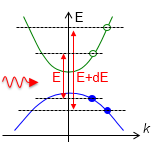
\includegraphics[scale=0.85]{ch5/image17}
		\captionof{figure}{ }
		\end{wrapfigure}		 
		Voyons ce qu'il en est pour les semi-conducteurs : à cause du continuum, le taux d'absorption 
		$r_a$ va s'exprimer par unité d'énergie et de volume. Sommons toutes les paires d'états 
		possédant une énergie entre $E$ et $E+\text{d}E$ 
		\begin{equation}
		{r_a}{\rm{d}}{{\rm{E}}_\omega } = \sum\limits_{{\rm{E < }}{{\rm{E}}_\omega } < {\rm{E + dE}}}
		 {\sigma {{\cal J}}} {f_i}(1 - {f_f}).1/V
		\end{equation}				 
		où $f_i$ est la probabilité d'occupation de l'état initial (doit être proche de 1) et 
		$1-f_f$ la probabilité que l'état final soit vide et $[\sigma  \propto | < {u_c}|x|{u_v} > 
		{|^2}$.\ \\
		
		Faisons deux hypothèses
		\begin{enumerate}
		\item La section efficace $\sigma$ est constante dans l'intervalle d'énergie 
		$[E,E+\text{d}E]$.
		\item La probabilité d'occupation initiale est donnée par la probabilité d'occupation dans 
		la bande de valence $f_i=f_v$ et la probabilité de l'état final est donnée par la probabilité
		d'occupation dans la bande de conduction $f_f=f_c$\footnote{Étant en situation de 
		quasi-équilibre, il faut tenir compte des quasi-énergies de Fermi.}.
		\end{enumerate}
		On peut alors écrire
		\begin{equation}
		\Rightarrow {r_a}{\rm{d}}{{\rm{E}}_\omega } = \sigma {{\cal J}}\frac{1}{V}\sum
		\limits_{{\rm{E < }}{{\rm{E}}_\omega } < {\rm{E + dE}}} {{f_v}(1 - {f_c})} 
		\end{equation}
		
		\newpage
		\begin{wrapfigure}[19]{l}{4cm}
%		\vspace{-5mm}
		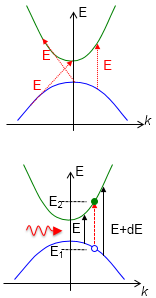
\includegraphics[scale=0.85]{ch5/image18}
		\captionof{figure}{ }
		\end{wrapfigure}
		Dans un semi-conducteur à gap direct, il y a plusieurs transitions possible pour une 
		différence d'énergie $E$. Il est nécessaire de conserver l'impulsion (à gauche, on considère
		éventuellement l'interaction avec un photon)
		\begin{equation}
		\hbar {\bf{k}}_i^e + \hbar {{\bf{k}}^{ph}} = \hbar {\bf{k}}_f^e
		\end{equation}
		Calculons l'impulsion d'un photon : $h\nu  = h\frac{c}{\lambda } \approx {{\rm{E}}_g}$. 
		Sachant que l'énergie de gap vaut à peu près 1eV, $\lambda\approx1.24\ \mu m$. Dès lors
		\begin{equation}
		{k^{ph}} = \frac{{2\pi }}{\lambda }\eta  \approx 15 \times {10^6}{\rm{ }}{{\rm{m}}^{{\rm{ -
		1}}}}
		\end{equation}
		La taille de la première zone de Brillouin est de l'ordre de 
		\begin{equation}
		\Delta k = \frac{{2\pi }}{a} \approx {10^{10}}{\rm{ }}{{\rm{m}}^{{\rm{ - 1}}}}
		\end{equation}				
		Il y a quatre ordre de grandeur entre les deux, une transition oblique n'est dès lors pas
		possible où alors il faut l'interaction d'une particule supplémentaire. Dans une 
		semi-conducteur à gap direct, le vecteur d'onde initial vaut le vecteur d'onde final
		\begin{equation}
		{\bf{k}}_i^e = {\bf{k}}_f^e
		\end{equation}
		Ce qui signifie que seulement les transitions verticales sont autorisées. Cela va simplifier
		la somme dans l'expression de $r_adE_\omega$
		\begin{equation}
		{r_a}{\rm{d}}{{\rm{E}}_\omega } = \sigma {{\cal J}}{f_v}({{\rm{E}}_1})(1 - {f_c}
		({{\rm{E}}_2}))\underbrace{\frac{1}{V}\sum\limits_{{\rm{E < }}{{\rm{E}}_\omega } < {\rm{E +
		dE}}} 1 }_{\text{d}N_t}
		\end{equation}
		où d$N_t$ est le nombre de paires électroniques par unité de volume avec le même vecteur 
		$\vec{k}$, séparés par une énergie dans l'intervalle $[E,E+\text{d}E]$ et $E_2-E_1=E_\omega
		=\hbar\omega$. On peut l'exprimer
		\begin{equation}
		{\rm{d}}{N_t} = p(\hbar \omega ){\rm{d}}{{\rm{E}}_\omega }
		\end{equation}
		où $p(\hbar\omega)$ est la densité d'états joints. Calculons son expressions dans l'espace
		réciproque\footnote{Résultat équivalent à celui obtenu pour la densité d'états.}
		\begin{equation}
		\Rightarrow {\rm{d}}{N_t} = \frac{2}{V}\frac{{4\pi {k^2}{\rm{d}}k}}{{{{(2\pi )}^3}/V}} =
		 \frac{{{k^2}{\rm{d}}k}}{{{\pi ^2}}}
		\end{equation}
		En utilisant l'approximation de bande parabolique pour la bande de valence et de conduction
		\begin{equation}
		\left.\begin{array}{ll}
		\DS{{\rm{E}}_1} &\DS= {{\rm{E}}_v} - \frac{{{\hbar ^2}{k^2}}}{{2{m_v}}}\vspace{2mm}\\
		\DS{{\rm{E}}_2} &\DS= {{\rm{E}}_c} + \frac{{{\hbar ^2}{k^2}}}{{2{m_c}}}
		\end{array}\right\}\quad\Rightarrow\quad {{\rm{E}}_\omega } = {{\rm{E}}_2} -
        {{\rm{E}}_1} = {{\rm{E}}_c} - {{\rm{E}}_v} + \frac{{{\hbar ^2}{k^2}}}{{2{m_c}}} +
		\frac{{{\hbar ^2}{k^2}}}{{2{m_v}}}
		\end{equation}
		En introduisant la masse effective réduite $\frac{1}{{{m_r}}} = \frac{1}{{{m_c}}} + \frac{1}
		{{{m_v}}}$ (traduisant la courbure des bandes)
		\begin{equation}
		{{\rm{E}}_\omega } = {{\rm{E}}_g} + \frac{{{\hbar ^2}{k^2}}}{{2{m_r}}}
		\end{equation}
		Effectuons la différentielle de cette expression ${\rm{d}}{{\rm{E}}_\omega } = {\hbar ^2}
		k{\rm{d}}k/{m_r}$. On trouve alors
		\begin{equation}
		{\rm{d}}{N_t} = \frac{{{m_r}}}{{{\hbar ^2}{\pi ^2}}}{\rm{d}}{{\rm{E}}_\omega }\sqrt {\frac{{({{\rm{E}}_\omega } - {{\rm{E}}_g})}}{{{\hbar ^2}}}2{m_r}}  = \frac{1}{{2{\pi ^2}}}{(\frac{{2{m_r}}}{{{\hbar ^2}}})^{3/2}}\sqrt {(\hbar \omega  - {{\rm{E}}_g})} {\rm{d}}{{\rm{E}}_\omega } = p({{\rm{E}}_\omega }){\rm{d}}{{\rm{E}}_\omega }
		\end{equation}
		Si $\hbar\omega$ est trop petit, la racine sera négative ce qui correspond à une transition 
		impossible (on serait dans la bande interdite). La $\sqrt{E}$ est (encore une fois) la 
		trace typique d'un objet massif tridimensionnel. Si $\hbar\omega>E_g$, la densité 
		d'état joint vaut alors\\
		
		\cadre{\begin{equation}
		p(\hbar \omega ) = \frac{1}{{2{\pi ^2}}}{(\frac{{2{m_r}}}{{{\hbar ^2}}})^{3/2}}\sqrt {(\hbar
		\omega  - {{\rm{E}}_g})} 
		\end{equation}}\ \\
		
		Notre taux d'absorption (différentiel) peut alors s'écrire
		\begin{equation}
		{r_a}{\rm{d}}{{\rm{E}}_\omega } = \sigma {{\cal J}}{f_v}(1 - {f_c})p({{\rm{E}}_\omega })
		{\rm{d}}{{\rm{E}}_\omega }
		\end{equation}
		En considérant toutes les énergies dans la bande d'énergie en question
		\begin{equation}
		{R_a} = \int {\sigma {{\cal J}}p({{\rm{E}}_\omega }){f_v}({{\rm{E}}_1})[1 - {f_c}
		({{\rm{E}}_{\rm{2}}})]{\rm{d}}{{\rm{E}}_\omega }} 
		\end{equation}
		Regardons comment varie les différents termes de $R_a$ et surtout la variation de la section
		efficace
		\begin{itemize}
		\item[$\bullet$] $\sigma  = B\hbar \omega g(\omega )/{v_g}$
		\begin{itemize}
		\item Dans un semi-conducteur, $g(\omega)$ est dominé par les collisions $\tau_0 \approx 
		ps\to\Delta\omega \approx 2\ THz$.
		\item A température ambiante $k_BT\approx1/40\ eV \to$ variation $f_c,f_v\approx 40$ THz.
		\end{itemize}
		\item[$\bullet$] Comme $40$ THz c'est lent\footnote{Pas du tout compris!} par rapport à 
		$\sigma$, on va remplacer $g(\omega)$ par un delta de Dirac pour les photons incidents
		d'énergie $\hbar\omega_0 \to g(\omega) = \delta(\omega-\omega_0)$
		\end{itemize}
		Dès lors (en négligeant l'incertitude aux collisions)
		\begin{equation}
		{R_a}({\omega _0}) = \frac{{B{\hbar ^2}{\omega _0}}}{{{v_g}}}{{\cal J}}p(\hbar {\omega
		 _0}){f_v}({{\rm{E}}_1})[1 - {f_c}({{\rm{E}}_{\rm{2}}})]
		\end{equation}
		
		\subsubsection{Taux d'émission stimulée}
		\begin{wrapfigure}[8]{l}{4cm}
		\vspace{-5mm}
		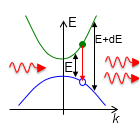
\includegraphics[scale=0.85]{ch5/image19}
		\captionof{figure}{ }
		\end{wrapfigure}		 
		Il faut que l'état final soit initialement vide à $E_1$. On définit de façon similaire au 
		taux d'absorption un taux de photons par unité d'énergie et de volume, $r_st$
		\begin{equation}
		{r_{st}}{\rm{d}}{{\rm{E}}_\omega } = \sigma {{\cal J}}{f_c}(1 - {f_v})p({{\rm{E}}_\omega
		 }){\rm{d}}{{\rm{E}}_\omega }
		\end{equation}
		On a remplacé $1-f_c$ par $f_c$ (l'état initial est occupé en conduction et vide en valence) 
		\begin{equation}
		{R_{st}}({\omega _0}) = \frac{{B{\hbar ^2}{\omega _0}}}{{{v_g}}}{{\cal J}}p(\hbar
		{\omega _0}){f_c}({{\rm{E}}_2})[1 - {f_v}({{\rm{E}}_{\rm{1}}})]
		\end{equation}				
		
		\subsubsection{Taux d'émission spontané}
		Ici, c'est plus difficile (notamment à cause du continuum d'énergie). Commençons par 
		introduire le taux d'émission spontané par unité de \textit{fréquence} $R_{sp,\omega}$.
		\begin{description}
		\item[$R_{sp,\omega}$d$\omega$] est le nombre de transitions radiatives par unité de 
		temps et de fréquence pour un photon possédant une fréquence angulaire \textbf{dans} 
		l'intervalle $[\omega,\omega+d\omega]$.
		\item[$p(\omega)$d$\omega$] est le nombre de transitions \textit{possibles} par unité de
		volume entre deux états séparés par une énergie dans l'intervalle $[\hbar\omega,\hbar(\omega
		+d\omega]$ (transitions verticales)
		\end{description}
		Commençons par calculer un élément de la transition (initialement, l'état final est vide)
		\begin{equation}
		{\rm{d}}{R_{sp,\omega '}} = {A_{21}}g(\omega ' - \omega ){f_c}[1 - {f_v}]p(\omega '){\rm{d}}
		\omega '
		\end{equation}
		S'il y a juste deux niveaux d'énergie, la photon émis à une énergie valant $E_2-E_1$, ce qui
		simplifie l'expression de $g(\omega)$ en un delta de Dirac\footnote{J'ai encore du mal à voir
		pourquoi.} : $g(\omega'-\omega) \approx \delta(\omega'-\omega)$. L'intégrale se calcule
		alors facilement (qui plus est, $A_{21} = 1/t_{sp}$)
		\begin{equation}
		{R_{sp,\omega }} = \int {{\rm{d}}{R_{sp,\omega '}}}  \approx \int {{A_{21}}\delta (\omega ' -
		\omega ){f_c}[1 - {f_v}]p(\omega '){\rm{d}}\omega '} 
		\end{equation}
		Le taux d'émission spontané par unité de fréquence à $\omega_0$ s'exprime alors\\
		
		\cadre{\begin{equation}
		{R_{sp,{\omega _0}}} = (1/{t_{sp}})p({\omega _0}){f_c}({{\rm{E}}_2})[1 - {f_v}({{\rm{E}}
		_{\rm{1}}})]
		\end{equation}}\ \\
		
		\textbf{Remarque.} On voit apparaitre $E_1$ et $E_2$ mais il faut se rappeler que ce choix
		n'est pas libre : la différence doit valoir $\hbar\omega_0$ et la transition doit être 
		constante. Il faut déterminer pour quelle valeur de $k$ l'énergie est séparée de $\hbar
		\omega_0$ mais si cette fréquence $\omega_0$ est fixée, ces énergies sont bien connues.
		
	\subsection{Absorption dans les semi-conducteurs à gap direct}
	Le but étant de faire un laser, il est nécessaire de déterminer les conditions d'absorption
	négatives et donc un gain positif. Soit un flux de photons $\mathcal{J}$ à énergie $\hbar	
	\omega_0$. En négligeant l'émission spontanée (la probabilité que l'émission spontanée contribue à
	l'émission laser est très faible). La variation de la densité de \textbf{photons} s'obtient en
	effectuant la différence entre ce qui est émis et ce qui est absorbé
	\begin{equation}
	\frac{{{\rm{d}}{n_p}}}{{{\rm{dt}}}} = {R_{st}} - {R_a} = \frac{{B\hbar }}{{{v_g}}}{{\cal J}}
	\hbar {\omega _0}p(\hbar {\omega _0})[{f_c}(1 - {f_v}) - {f_v}(1 - {f_c})]
	\end{equation}
	\begin{wrapfigure}[9]{l}{5cm}
	\vspace{-6mm}
	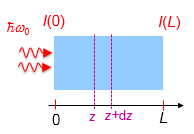
\includegraphics[scale=0.9]{ch5/image21}
	\captionof{figure}{ }
	\end{wrapfigure}
	Considérons cette fois-ci la variation spatiale de la densité de photons que nous multiplions 
	par $v_g$
	\begin{equation}
	{v_g}\frac{{{\rm{d}}{n_p}}}{{{\rm{dz}}}} = \frac{{B\hbar }}{{{v_g}}}p(\hbar {\omega _0})[{f_c} -
	 {f_v}]I
	\end{equation}
	où nous avons utilisé $I = \mathcal{J}\hbar\omega_0$ et $\mathcal{J} = n_pv_g$. Il ne reste 
	que la différence entre $f_c$ et $f_v$ mais nous avons surtout fait apparaître l'intensité. On en
	extrait l'ED suivante
	\begin{equation}
	\frac{{{\rm{d}}I}}{{{\rm{dz}}}} = \frac{{B{\hbar ^2}{\omega _0}}}{{{v_g}}}p(\hbar {\omega _0})
	[{f_c} - {f_v}]I =  - \alpha I
	\end{equation}
	Par identification, on trouve le fameux coefficient symbolisant les pertes\\
	
	\cadre{\begin{equation}
	\alpha  = \frac{{B{\hbar ^2}{\omega _0}}}{{{v_g}}}p(\hbar {\omega _0})[{f_v}({{\rm{E}}_1}) - {f_c}
	({{\rm{E}}_2})]
	\end{equation}}\ \\
	
	Si le semi-conducteur est intrinsèque (ou faiblement dopé), cela signifie que la probabilité 
	d'occupation à l'état électrique $E_2$ est à peu près nul : à l'équilibre thermique, dans un 
	matériau faiblement dopé, la bande de conduction est essentiellement vide mais elle vaut à peu
	près 1 dans la bande de valence
	\begin{equation}
	{f_c}({{\rm{E}}_2}) \approx 0,\qquad\qquad\qquad\rm{  }{f_v}({{\rm{E}}_1}) \approx 1
	\end{equation}
	Dès lors
	\begin{equation}
	\Rightarrow \alpha (\hbar {\omega _0}) = \frac{{B{\omega _0}}}{{2\hbar {\pi ^2}{v_g}}
	}{(2{m_r})^{3/2}}\sqrt {(\hbar {\omega _0} - {{\rm{E}}_g})} \qquad\qquad
	(\hbar\omega_0>E_g)
	\end{equation}
	Le coefficient d'absorption montre un seuil d'énergie $\hbar\omega=E_g$. Il augmente comme une 
	fonction racine, tout comme la densité d'états joints.
	\begin{center}
	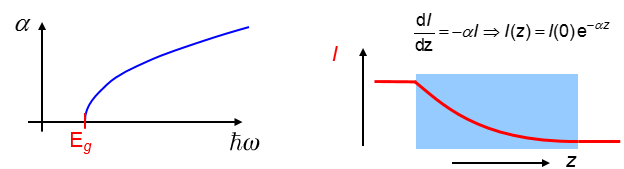
\includegraphics[scale=0.6]{ch5/image22}
	\captionof{figure}{ }
	\end{center}	
	Ce résultat décrit assez bien la réalité (cf. slides 26-27).
		
	
	\subsection{Saturation de l'absorption}
	\begin{wrapfigure}[11]{r}{3.4cm}
	\vspace{-20mm}
	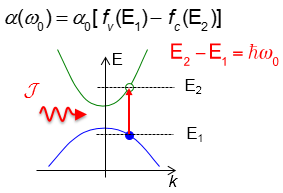
\includegraphics[scale=0.6]{ch5/image23}
	\captionof{figure}{ }
	\end{wrapfigure}	
	Supposons que l'on soit en présence un faible flux de photon $\mathcal{J}$. Dans ce cas, la 
	densité électronique est proche de l'équilibre thermique ce qui implique que 
	\begin{equation}
	\alpha(\omega_0) \approx \alpha_0
	\end{equation}
	
	Si cette fois la flux de photon $\mathcal{J}$ est important, il va y avoir thermalisation des 
	électrons excités dans la bande de conduction et des trous dans la bande de valence : 
	$E_{fc}, E_{fv} \neq \mu$\footnote{Pq?}. Les distributions sont données par
	\begin{equation}
	{f_c}({{\rm{E}}_2}) = 1/(1 + \exp [({{\rm{E}}_2} - {{\rm{E}}_{fc}})/{k_{\rm{B}}}T]),\qquad
	{f_v}({{\rm{E}}_1}) = 1/(1 + \exp [({{\rm{E}}_1} - {{\rm{E}}_{fv}})/{k_{\rm{B}}}T])
	\end{equation}
	La densité électronique s'obtient de façon similaire à ce qui a été vu précédemment
	\begin{equation}
	{n_e} = \int {{f_{c,v}}({\rm{E}})\rho ({\rm{E}}){\rm{dE}}} 
	\end{equation}
	Comme l'absorption dépend de la différence entre $f_v$ et $f_c$\footnote{$\alpha  = 
	\frac{{B{\hbar ^2}{\omega _0}}}{{{v_g}}}p(\hbar {\omega _0})[{f_v}({{\rm{E}}_1}) -
	{f_c}({{\rm{E}}_2})]$} et qu'elles tendent toutes les deux vers $1/2$ lorsque le flux est très
	intense, l'absorption tend vers zéro: $\alpha\to0$.\\
	
	On dit donc que l'absorption est \textbf{saturable} : elle n'est pas la même pour un flux de 
	photons faible que pour un flux important. Quand le flux est important, l'absorption devient
	faible d'où le \textit{saturable}. On écrit alors
	\begin{equation}
	\alpha  = \frac{{{\alpha _0}}}{{1 + {\cal J}/{{\cal J}_s}}}
	\end{equation}
	où $\mathcal{J}_s$ est le flux de saturation.\\
	
	\textsc{Application : génération d'impulsions courtes}\\
	\begin{wrapfigure}[6]{l}{8cm}
	\vspace{-5mm}
	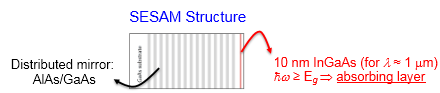
\includegraphics[scale=0.6]{ch5/image26}
	\captionof{figure}{ }
	\end{wrapfigure}
	Cette saturation a une application : les miroirs "SESAM". On considère un matériau pour lequel
	l'énergie du gap est inférieur à l'énergie des photons de sorte que ceux-ci soient absorbés. En 
	alternance, sur ce matériau, on crée une structure périodique de $AlAs/GaAs$ qui ont des 
	indices de réfraction différents :l'énergie du gap est cette fois-ci supérieur à celle des 
	photons ($E_g\geq\hbar\omega)$. \\
	
	Lorsqu'un flux de photon va passer dans cette structure, il va y avoir une réflexion partielle
	à chaque variation de l'indice de réfraction\footnote{Lorsque l'on passe d'un indice plus grand à
	plus petit et inversement, le signe des indices de réflexion sont inversés. Le signe est par
	contre toujours positif pour la réflexion.}

	\begin{center}
	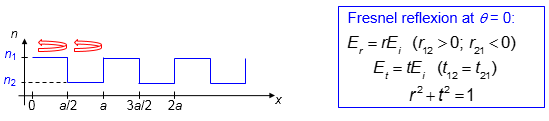
\includegraphics[scale=0.8]{ch5/image24}
	\captionof{figure}{ }
	\end{center}
	Sans les réflexions secondaires
	\begin{equation}
	R =  + r{{\rm{e}}^{2ika/2}} - r{t^2}{{\rm{e}}^{4ika/2}} + r{t^4}r{{\rm{e}}^{6ika/2}} - r{t^6}
	{{\rm{e}}^{8ika/2}} + \dots
	\end{equation}		
	En analysant les séries positives et négatives, il est possible de trouver
	\begin{equation}
	(...) = \frac{1}{{1 - {t^4}{{\rm{e}}^{4(ika/2)}}}}\qquad\qquad |t|^2<1
	\end{equation}		
	Avec un traitement des réflexions multiples, on trouve comme coefficient (sans justification)
	\begin{equation}
	R = \frac{{{r^2}{{\rm{e}}^{ika}} - {r^2}{t^2}{{\rm{e}}^{2ika}}}}{{1 - {t^4}{{\rm{e}}^{4(ika/2)}}}}
	\end{equation}
	Ce coefficient possède une résonance : la \textit{réflexion de Bragg} (réflexion totale)
	\begin{equation}
	ka = m\pi\qquad\Rightarrow\qquad |R|=1
	\end{equation}
	

	\begin{wrapfigure}[8]{l}{9cm}
	\vspace{-5mm}
	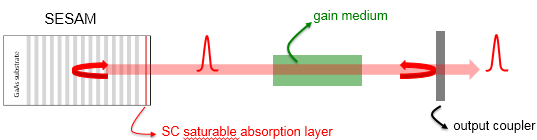
\includegraphics[scale=0.6]{ch5/image25}
	\captionof{figure}{ }
	\end{wrapfigure}
	Sur base de ce principe, considérons le setup ci-contre.
	Ce setup permet de générer des impulsions très courtes (génération par bloquage de mode). Il va 
	préférentiellement pulser qu'émettre en continu car quand l'impulsion traverse l'élément saturable 
	il y aura moins de pertes que dans le cas continu.
	
	\newpage
	\subsection{Gain optique}
	Après avoir regardé l'absorption, il serait intéressant que celle-ci soit négative afin d'avoir
	du gain. Considérons $\alpha$ et l'équation de Beer-Lambert
	\begin{equation}
	\alpha  = \frac{{B{\hbar ^2}{\omega _0}}}{{{v_g}}}p(\hbar {\omega _0})[{f_v}({{\rm{E}}_1}) - {f_c}({{\rm{E}}_2})] =  - {\cal G}\qquad\Rightarrow\qquad
	\frac{{{\rm{d}}I}}{{{\rm{dz}}}} =  - \alpha ({\omega _0})I =  + {{\cal G}}I
	\end{equation}
	La seul façon pour avoir un positif est que le crochet soit négatif (comme $\alpha=-\mathcal{G}$)
	\begin{equation}
	\Leftrightarrow [{f_v}({{\rm{E}}_1}) - {f_c}({{\rm{E}}_2})] \le 0
	\end{equation}
	où ${{\rm{E}}_2} - {{\rm{E}}_1} = \hbar {\omega _0}$, ssi
	\begin{equation}
	\Leftrightarrow {f_c}({{\rm{E}}_2}) \ge {f_v}({{\rm{E}}_1})
	\end{equation}
	En explicitant les distributions
	\begin{equation}
	(1+\exp\left[(E_2-E_{fc})/k_BT\right])^{-1} \geq (1+\exp\left[(E_1-E_{fv})/k_BT\right])^{-1}
	\end{equation}
	Si et seulement si
	\begin{equation}
	{{\rm{E}}_2} - {{\rm{E}}_{fc}} \le {{\rm{E}}_1} - {{\rm{E}}_{fv}} \Leftrightarrow {{\rm{E}}_2} -
	 {{\rm{E}}_1} \le {{\rm{E}}_{fc}} - {{\rm{E}}_{fv}}
	\end{equation}
	On en tire la \textbf{relation de Bernard-Duraffourg}\\
	
	\cadre{\begin{equation}
	\hbar {\omega _0} \le {{\rm{E}}_{fc}} - {{\rm{E}}_{fv}} = \Delta {{\rm{E}}_f}
	\end{equation}
	Il s'agit de la condition nécessaire pour avoir un taux d'émission stimulée plus grand qu'un 
	taux d'absorption.}\ \\
	
	Il s'agit de l'équation équivalente à l'inversion de population pour un semi-conducteur. Il 
	faut qu'il y ai en effet plus d'émission stimulée (recombinaison paire électron/trou) que de 
	création de paires (signifie qu'il y a plus de chance de trouver des électrons dans la bande 
	de valence que de conduction).
	
	\begin{center}
	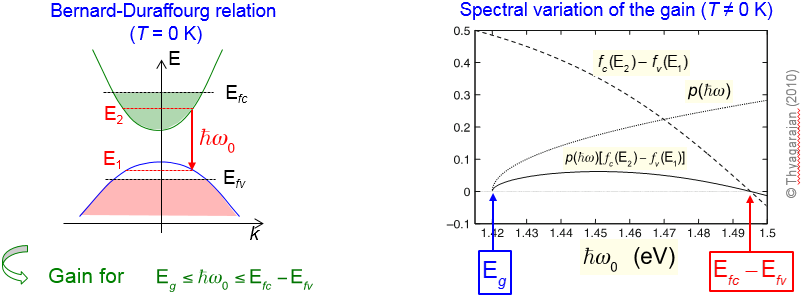
\includegraphics[scale=0.6]{ch5/image27}
	\captionof{figure}{ }
	\end{center}
	Si on regarde plus en détail le gain, on remarque qu'il dépend (spectralement) de la différence 
	entre les deux énergies.\\
	
	\textsc{Application : injections de porteurs dans une jonction pn}\\
	\begin{wrapfigure}[10]{l}{4.5cm}
	\vspace{-5mm}
	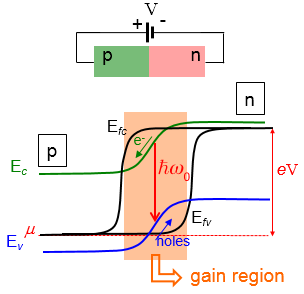
\includegraphics[scale=0.5]{ch5/image28}
	\captionof{figure}{ }
	\end{wrapfigure}
	Lorsque l'on applique une tension sur une telle jonction, un "plateau" va descendre et l'autre 
	monté de sorte a avoir une "inversion" du graphique (voir ci-contre) : les électrons vont pouvoir
	descendre plus bas et les trous monter plus haut : émission d'un photon et recombinaison. La 
	condition de Bernard-Duraffourg devient alors 
	\begin{equation}
	{{\rm{E}}_g} \le \hbar {\omega _0} \le {{\rm{E}}_{fc}} - {{\rm{E}}_{fv}} = eV
	\end{equation}
	Comme annoncé, le spectre de gain/absorption est fonction de la densité de porteurs libres
	\begin{center}
	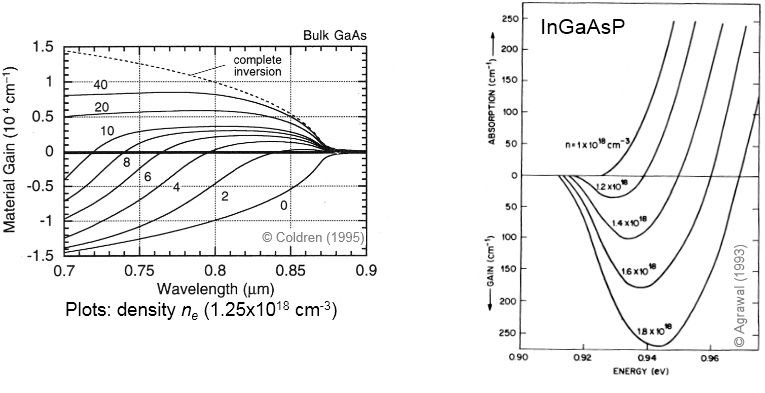
\includegraphics[scale=0.35]{ch5/image29}
	\captionof{figure}{ }
	\end{center}
	La courbe 0 (ci-dessus, à gauche) correspond au cas ou aucune charge n'est injectée dans le 
	semi-conducteur : il  n'y a que de de l'aborption. Plus on augmente l'injection, plus le 
	décolement est important et il est possible d'avoir un gain et plus celle-ci augmente, plus 
	le gain devient important. En résumé, lorsque la densité de porteurs augmente
	\begin{enumerate}
	\item La largeur spectrale du gain augmente
	\item La valeur maximal du gain augmente
	\item La fréquence optique pour laquelle le gain est maximal augmente
	\end{enumerate}
	

\newpage
\section{Transition électroniques non radiatives}
Il est possible d'avoir des phénomènes de recombinaison électron/trou sans émission de photons. On 
pourrait (logiquement) considérer que si c'est le cas, il y a émission de phonons. Or, pour passer
le gap ($E_g\approx 1\ eV$) 30 à 40 phonons sont nécessaire (ayant une énergie de 1/40 eV à 
température ambiante). La probabilité qu'ils interagissent tout en même temps est faible mais c'est
totalement faisable par niveaux successifs\dots à cause des défauts!

	\subsection{Recombinaisons en surface et par défauts}
	\begin{wrapfigure}[8]{l}{4.5cm}
	\vspace{-5mm}
	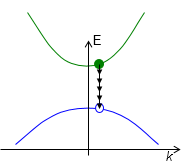
\includegraphics[scale=0.6]{ch5/image30}
	\captionof{figure}{ }
	\end{wrapfigure}
	On peut considérer les défauts (dislocations ou ponctuels) ainsi que les surfaces (plus de 
	périodicité, impuretés) mais localement, il y a bien toujours un continuum d'état électronique
	dans la bande interdite. \\
	
	Définissons le taux de recombinaison $R=A_{nr}n_e$. Celui-ci est logiquement lié à la densité
	électronique (plus il y a d'espèce présentes, plus il y a des chances d'avoir une 
	recombinaison). Le coefficient de proportionnalité est $A_{nr}$ :
	\begin{itemize}
	\item[$\bullet$] $A_{nr}\propto $ densité de défauts
	\item[$\bullet$] $A_{nr}\propto $ aire de la surface
	\end{itemize}
	Pour des applications optiques, il faut donc avoir un semi-conducteur extrêmement pur avec 
	une zone active et pas de surface libre. Aujourd'hui, on parvient à avoir une densité de 
	défaut négligeable. Le problème apparait lorsque l'on utilise le structure pour avoir de la
	lumière. Par exemple, il faut mettre pas mal de tension sur une jonction $pn$ ce qui crée 
	un échauffement, responsable de l'apparition de défauts. Ces défauts sont des centres de 
	recombinaison non radiatifs.
	
	
	\subsection{Recombinaisons d'Auger}	
	\begin{wrapfigure}[10]{l}{7cm}
	\vspace{-5mm}
	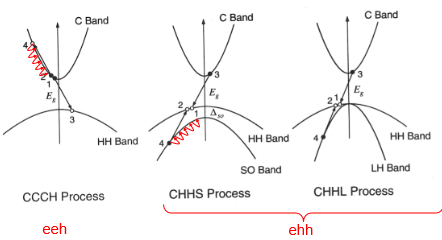
\includegraphics[scale=0.6]{ch5/image31}
	\captionof{figure}{ }
	\end{wrapfigure}		
	Il s'agit d'un processus de recombinaison où l'énergie ne va pas dans un photon, mais dans 
	l'excitation d'une charge ou d'un trou. Par exemple, l'électron passe de la bande de 
	conduction à celle de valence (recombinaison) et la différence d'énergie est cédée à un 
	électron qui va se retrouver beaucoup plus haut dans la bande de conduction pour enfin 
	se thermaliser et redescendre. Notons que le même processus peut être possible avec un trous 
	(il peut même y avoir un changement de bande).\\
	
	Il s'agit du processus non radiatif dominant dans les semi-conducteurs. Comme vu sur le schéma
	ci-dessus à gauche, il se divise en deux processus
	\begin{enumerate}
	\item \textit{Processus eeh} : excite un électron plus haut dans la bande de conduction
	\item \textit{Processus ehh} : excite un trou pronfondément danslabande de valence.
	\end{enumerate}
	La thermalisation se fait par émission successives de phonons (conservation de l'énergie et
	de l'impulsion). Le taux de recombinaison d'Auger $R_A$ varie selon le type de l'interaction
	\begin{equation}
	R_A^{{\rm{eeh}}} \propto {n_e}^2{n_h},\qquad\qquad R_A^{{\rm{ehh}}} \propto {n_e}n_h^2
	\end{equation}
	La densité de l'espèce excitée se retrouve mise au carrée. Trois cas possibles
	\begin{enumerate}
	\item SC intrinsèque ($n_e=n_h$)
	\begin{equation}
	{R_A} = C{n_e}^3 = \frac{{{n_e}}}{{{\tau _A}}}
	\end{equation}
	où $\tau _A^{ - 1} = Cn_e^2$. On a tendance à écrire $cn_e^3$ comme un nombre de charge par 
	unité de volume divisé par un temps caractéristique : il s'agit du \textit{temps de recombinaison
	d'Auger}\footnote{Ce n'est pas une constante, mais $n_e^*c^{te}$.}.
	\item SC dopé $n$ : processus dominant \textit{eeh}
	\begin{equation}
	R_A^{{\rm{eeh}}} =  - \frac{{\rm{d}}}{{{\rm{d}}t}}{n_e} = {C^{{\rm{eeh}}}}{n_e}^2{n_h} = \frac{{{n_e}}}{{\tau _A^{{\rm{eeh}}}}}
	\end{equation}
	\item SC dopé $p$ : processus dominant \textit{ehh}
	\begin{equation}
	R_A^{{\rm{ehh}}} =  - \frac{{\rm{d}}}{{{\rm{d}}t}}{n_h} = {C^{{\rm{ehh}}}}{n_h}^2{n_e} = \frac{{{n_h}}}{{\tau _A^{{\rm{ehh}}}}}
	\end{equation}
	\end{enumerate}
	
	
	
\section{Matériaux et structures pour les diodes lasers}
Nous allons ici voir quels sont les \textit{bons} matériaux pour fabriquer des sources lasers : la 
condition de Bernard va en effet nous imposer une structure particulière.

	\subsection{Taux de recombinaison total}
	Un matériau est bon s'il maximise les recombinaisons électrons-trous qui génèrent des photons. 
	Plaçons-nous dans le cas d'une diode électroluminescente : son taux radiatif est l'intégrale 
	sur les fréquences du taux de recombinaison spontané
	\begin{equation}
	{R_{sp}} = \int {{R_{sp,\omega }}{\rm{d}}\omega } 
	\end{equation}
	Procédons à une approche phénoménologique : pour avoir recombinaison il faut avoir un électron 
	et un trou. Le taux de recombinaison doit être proportionnel aux densités de ces charges libres. 
	En définissant le coefficient de proportionnalité $B$ comme le \textit{coefficient de 
	recombinaision bimoléculaire}, on note
	\begin{equation}
	{R_{sp}} = B({n_e}){n_e}{n_h}
	\end{equation}
	Pour un SC intrinsèque
	\begin{equation}
	{R_{sp}} =  - {(\frac{{{\rm{d}}{n_e}}}{{{\rm{d}}t}})_{Rad}} = B({n_e}){n_e}^2 = \frac{{{n_e}}}
	{{{\tau _R}}}
	\end{equation}
	où $\tau_R$ est le temps de vie radiatif. Il ne faut cependant pas oublier les recombinaisons 
	d'Auger. On en tient compte en définissant $R_{tot}$ :
	\begin{equation}
	{R_{tot}} =  - (\frac{{{\rm{d}}{n_e}}}{{{\rm{d}}t}}) = {R_R} + {R_A} = \frac{{{n_e}}}{{{\tau _R}}}
	 + \frac{{{n_e}}}{{{\tau _A}}}
	\end{equation}
	où $\tau _R^{ - 1} = B{n_e}$ et $\tau _A^{ - 1} = C{n_e}^2$. Pour former une diode laser, il est
	nécessaire d'avoir un temps de recombinaison radiatif bien plus court que le temps de 
	recombinaison d'Auger: $\tau_R \ll \tau_A$. Le tableau comparatif ci-dessous compare ces temps 
	de vie
	\begin{center}
	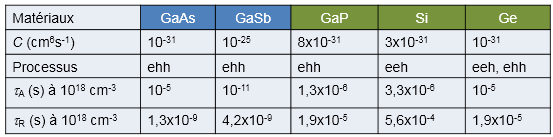
\includegraphics[scale=0.8]{ch5/image32}
	\captionof{table}{Coefficients données pour des SC intrinsèques. Bleu signifie à gap direct et 
	vert à gap indirect.}
	\end{center}

	\begin{wrapfigure}[15]{l}{5.5cm}
%	\vspace{-5mm}
	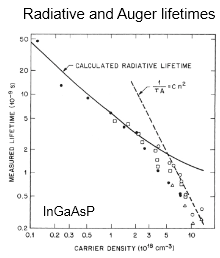
\includegraphics[scale=0.8]{ch5/image33}
	\captionof{figure}{ }
	\end{wrapfigure}
	Pour le $GaAs$, les recombinaisons sont essentiellement radiatives. Pour le $GaSb$ l'écart entre
	les deux temps caractéristique est faible mais par malchance, le processus Auger est très 
	efficace dans ce matériau. Pour les trois SC à gap indirect\footnote{Généralité visiblement} il
	n'est pas non plus possible d'en faire une diode laser.\\
	
	Pour le \textit{GaAs}, on retrouve $\tau_A\ll \tau_R$ : il s'agit d'un bon matériau 
	pourvu que la densité des porteurs n'est pas trop élevée ($\tau_A^{-1}=Cn_e^2$). 
	Il y a donc une limitation de la concentration de dopage ($p$ ou $n$) et des charges libres
	injectés de sorte que le processus de recombinaison majeur soit la radiative. Un bon matériau 
	pour une diode laser est ainsi un SC à gap direct, dopé seulement dans la région active avec 
	une faible concentrations te défauts et d'impuretés.
	
	
	\subsection{Longueur d'onde d'émission}	
	\begin{wrapfigure}[15]{r}{5.5cm}
	\vspace{-5mm}
	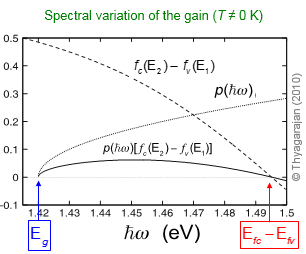
\includegraphics[scale=0.8]{ch5/image34}
	\captionof{figure}{ }
	\end{wrapfigure}
	Si l'on observe la variation spectrale du gain, on peut se rendre compte que l'on obtient un 
	gain positif pour des énergies proche de la bande électronique et légèrement au dessus de 
	celle-ci. La fréquence d'émission sera alors directement liée à l'énergie du gain
	\begin{equation}
	\text{Émission à }\ \omega = E_g/\hbar
	\end{equation}
	La composition chimique semi-conductrice est également choisie en fonction de la longueur d'onde 
	d'émission ciblée. Le ratio suivent est alors assez pratique
	\begin{equation}
	\frac{\lambda }{{1{\rm{ }}\mu {\rm{m}}}} = \frac{{1.24}}{{{\rm{E/1 eV}}}}
	\end{equation}
	Les slides 48 et 49 donnent des exemples d'applications et comment les propriétés chimiques 
	peuvent influencer la longueur d'onde émise.\\
	
	Un autre paramètre a une grande importance : le paramètre de maille (constante de réseau) $a$.
	Comme la structure du 	laser est constitué de jonctions entre semi-conducteurs, la constante de
	réseau $a$ doit être très proche pour les deux alliages en contact afin d'éviter les défauts 
	ponctuels et les dislocations 
	\begin{equation}
	\dfrac{\Delta a}{a} < 0.1\%
	\end{equation}
	Par exemple, considérerons deux matériau semi-conducteurs
	\begin{equation}
	\left.\begin{array}{ll}
	AlAs &: a_1\\
	GaAs &: a_2
	\end{array}\right\} \to Al_xGa_{1-x}As: a \approx xa_1+(1-x)a_2
	\end{equation}
	

	\begin{wrapfigure}[12]{l}{7cm}
	\vspace{-5mm}
	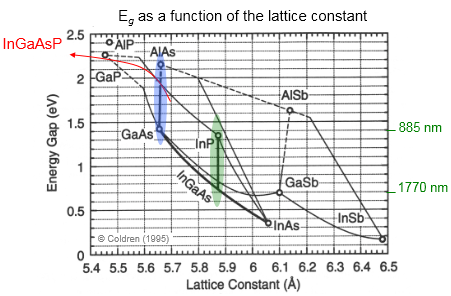
\includegraphics[scale=0.6]{ch5/image35}
	\captionof{figure}{ }
	\end{wrapfigure}
		
	Dans le cas de $Al_xGa_{1-x}As$, $a_1 = 5.66\ \AA, a_" = 5.6533\ \AA$ : il s'agit d'un aliage de
	choix pour les applications optique, tant la variation de la constante de réseau est proche! 
	La jonction \textit{AlGaAs/GaAs} permet de créer des diodes lasers entre 720 et 850 nm.\\
	
	En pointillé ci-contre les gaps indirects et en traits pleins les gaps directs. Ce graphique 
	permet de choisir un bon alliage : il faut un gap direct et une faible variation (au revoir 
	\textit{AlAl/AlSb}) et une (très) faible variation du paramètre de maille (au revoir 
	\textit{AlSb/GaSb}). On voit que les diodes laser $AlAs/GaAs$ sont en effet possibles : si on
	bloque le rapport $x/y$ on se balade sur un trait vertical et on va pouvoir modifier l'énergie 
	de gap (toujours drect) pour jouer sur la longueur d'onde émise!

	
	\subsection{Structures des diodes laser}
		\subsubsection{Laser à homojonction}
 		\begin{wrapfigure}[7]{r}{6.5cm}
		\vspace{-5mm}
		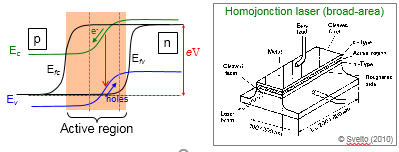
\includegraphics[scale=0.6]{ch5/image36}
		\captionof{figure}{ }
		\end{wrapfigure} 	
 		La première structure qui vient à l'esprit est une simple jonction \textit{pn} : il suffit
 		de lui appliquer une tension supérieur à celle du gap. Ceci cause une inversion des courbes
 		par rapport à l'équilibre permettant aux électrons de descendre et aux trous de monter (ils
 		pourront passer librement, il n'y a en effet pas de barrière de potentiel). On va alors 
 		s'arranger pour avoir un gain (il faut que la différence entre les deux quasi niveaux de Fermi
 		soit plus grande que l'énergie du gap). Il reste à former une cavité, que l'on considère 
 		Fabry-Perot avec un miroir où $R=0.35$ : faible, mais le gain est tellement important qu'il 
 		n'y a pas de soucis. Pour éviter que ça lase dans la "mauvaise" direction on va scier la 
 		surface pour introduire des rugosités : beaucoup de pertes, empêchant le lasage.\\
 		
 		\begin{wrapfigure}[9]{l}{5cm}
		\vspace{-5mm}
		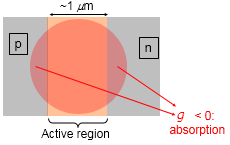
\includegraphics[scale=0.8]{ch5/image37}
		\captionof{figure}{ }
		\end{wrapfigure}
 		C'est relativement simple, mais il y a pleins d'éléments qui font que ça ne va pas aussi 
 		bien se passer que prévu. Le premier souci est la tension importante à fournir (quelques 
 		volts, bien au delà du seuil de 0.7 V apparaissant dans la caractéristiques des diodes, 
 		donnant lieu à un courant important). Un autre problème est la largeur de la bande active
 		(zone de déplétion) qui n'est pas bien définie (dépend de la tension appliquée) : diffusions
 		de porteurs minoritaires causant un étalement du gain (mais pas infini car pas de gain en 
 		dehors). Le souci est qu'en dehors de la zone active il y a absorption : pertes internes 
 		élevées. Comme un courant important crée un échauffement (création de défaut ; effet de 
 		vieillissement), cette strucutre n'est pas utilisée pour les lasers.
 		
 		\newpage
 		\subsubsection{Laser à double hétéro-jonction}
 		 \begin{wrapfigure}[8]{l}{9cm}
		\vspace{-5mm}
		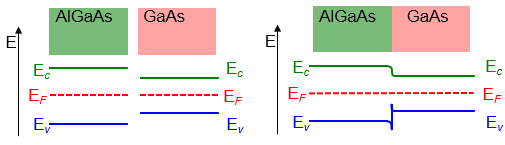
\includegraphics[scale=0.6]{ch5/image38}
		\captionof{figure}{ }
		\end{wrapfigure}
 		La solution pour ce chauffage est d'utiliser les hétéro-jonctions : on va mettre en contact
 		deux semi-conducteurs différents, possédant un gap différent. C'est possible, si les 
 		paramètres de mailles sont très proches.\\
 		\ \\
 		
 		Comme faire juste une hétéro-jonction ne suffit pas, on va en faire des doubles\footnote{Il 
 		va falloir ré-expliquer\dots} et de part et d'autre d'un matériau semi-conducteur : une du 
 		côté $p$ et une autre du côté $n$ avec un gap plus important, le but étant de piéger les
 		charges dans la région centrale (active). 
 		De plus, on veut être en condition d'inversion mais avec des barrières de potentiel 
 		empêchant de traverser totalement (premier schéma, \textit{before contact}). \\
 		
 		Lorsque l'on applique une tension passante, il faut bien évidemment que la différence entre 
 		les deux niveaux de Fermi soit supérieure à l'énergie du gap (pour avoir un gain). En faisant 
 		ça, on se retrouve avec une marche de potentiel (schéma de droite, tout en haut) que l'on 
 		avait pas avant, empêchant les électrons de passer de la région $n$ à $p$ et de même pour 
 		les trous : ils sont piégé dans la région centrale\footnote{???}.
	
		\begin{center}
		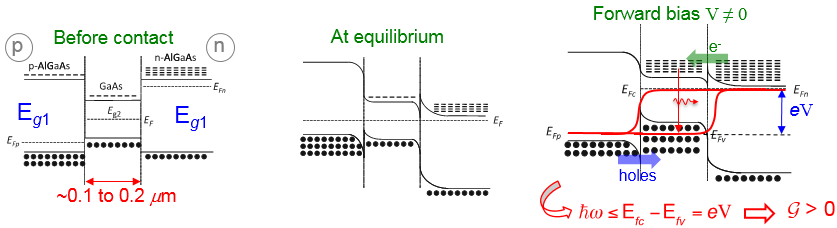
\includegraphics[scale=0.7]{ch5/image39}
		\captionof{figure}{ }
		\end{center}
	
		Une telle strucutre se met facilement en place avec des de fils électriques. L'avantage de
		cette méthode est que les porteurs sont confinés dans la zone active, tout en limitant la
		tension à metre grâce aux barrières. Un autre avantage vient du fait qu'une modification du 
		gap cause une modification de l'indice de réfaction : le profil de cet indice sera plus 
		élevé dans la zone active. Au centre de la zone active, si certains rayons sont rasants 
		à la "paroi", ils vont être totalement réfléchi et confiné dans cette région d'indice plus
		élevé : structure "guidante" provoquant un confinement du champ EM. De plus, comme 
		l'énergie du photon est $E_{g2} < h\nu < E_{g1}$ il n'y aura pas d'absorption.	
		\begin{center}
		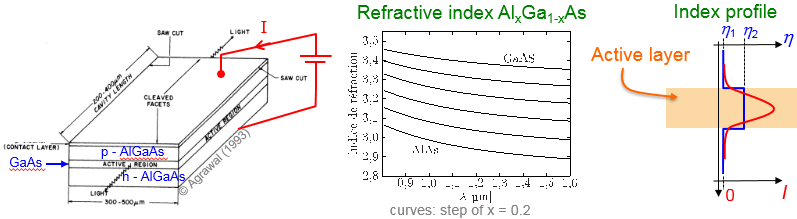
\includegraphics[scale=0.7]{ch5/image40}
		\captionof{figure}{ }
		\end{center}
	
	\begin{wrapfigure}[6]{l}{9cm}
	\vspace{-5mm}
	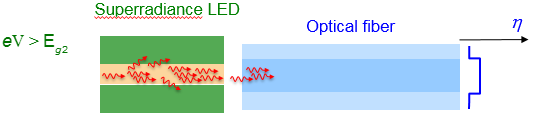
\includegraphics[scale=0.6]{ch5/image41}
	\captionof{figure}{ }
	\end{wrapfigure}	
		Dans certains cas, il peut y avoir une émission mais non laser car celle-ci n'est pas 
		confinée : on parle de \textbf{super-radiance}. Si on polarise la double hétéro-jonction 
		mais en dessous du seuil laser, cela ne lasera pas. Cependant, si la tension appliquée est
		supérieure à celle du gap, la zone centrale possèdera tout de même un gain (mais trop faible
		pour que ça lase). Un photon dans cette zone va rester dans la structure guidante et être
		amplifié : donne lieu à une petite fraction réfléchie qui va circuler à l'intérieur. Il en
		résulte un champ plus cohérent que l'émission spontannée mais moins qu'un laser : c'est 
		un cas "intermédiaire". On peut utiliser ça comme "source de bon marché" pour des applications
		en télécommunications à courtes distances.\\
		
	\begin{wrapfigure}[11]{r}{5cm}
	\vspace{-5mm}
	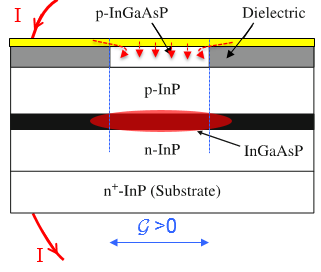
\includegraphics[scale=0.6]{ch5/image42}
	\captionof{figure}{ }
	\end{wrapfigure}	
		On l'a compris, avoir un effet de guidage est intéressant: il faut confiner la lumière au 
		centre de la région active dans la direction de la jonction (et pas dans la direction 
		transverse, c'est-à-dire la partie "plane" de plan de la couche active)\footnote{Ceci causera
		des effets de diffraction et une inhomogénéité du courant (laser multimode transverse, cf. 
		laboratoires).}. Pour se faire on peut guider soit par gain, soit par saut d'indice.\\
		
		Par gain c'est assez simple : on limite spatialement la zone où $\mathcal{G}>0$ en retirant
		une partie du matériau. Comme le gain est limité, il en est de même pour le faisceau laser. 
		Notons que l'extension spatiale de la région à gain dépend du courant $I$.\\
		
		Pour le guidance par saut d'indice, deux choix
		\begin{enumerate}
		\item Guidage faible : zone d'indice de réfraction supérieur près de la zone active ($\Delta
		\eta_{eff} \approx 10^{-2}$). Le confinement latéral dépend du courant $I$ comme la zone
		active dépend de l'indice de réfraction qui lui-même varie avec la densité de porteurs.
		\begin{center}
			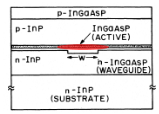
\includegraphics[scale=0.8]{ch5/image43}
	\captionof{figure}{ }
		\end{center}
		\item Guidage fort : tous les matériau \textit{autour} de la zone active sont plus faibles 
		(il suffit de changer la composition chimique) : lorsque le courant arrive sur la zone rouge, 
		il est obliger de se déplacer vers la zone active (pareil pour les trous "en dessous" de 
		cette zone). Ici les sauts d'indices peuvent être bien élevés ($\approx 0.2$) ce qui 
		permet de bien confiner la lumière.
		\end{enumerate}
		\begin{center}
			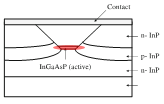
\includegraphics[scale=0.8]{ch5/image44}
	\captionof{figure}{ }
	Ce genre de structure est largement rencontrée en télécommunication pour des applications 
	de guidage monomode : il y a en effet un bon couplage entre la source laser et la fibre optique.
		\end{center}	
	
	
	
\section{Modèle simple des lasers à semi-conducteurs}
	\subsection{Équation de bilan d'une diode laser}
	Considérons que la zone active est un semi-conducteur intrinsèque $n_e\approx n_t$ : c'est la
	seule équation pour les porteurs et l'équation de bilan de la densité électrique $n_e$. 
	Soit le taux de recombinaison des porteurs
	\begin{equation}
	\frac{{{\rm{d}}{n_e}}}{{{\rm{d}}t}} = {R_{{\rm{gen}}}} - {R_{{\rm{rec}}}}
	\end{equation}
	Le \textit{taux de génération} des porteurs dans la région active est donné par
	\begin{equation}
	{R_{{\rm{gen}}}} = {\eta _i}\frac{{I}}{{qV}} + {R_A}
	\end{equation}
	où $\eta_i$ est le rendement quantique interne, c'est-à-dire la fraction du courant qui génère
	des porteurs dans la zone active de volume $V$ et $q$ un élément de charge. Pour la recombinaison,
	nous avions la contribution des radiatives et celles de Auger
	\begin{equation}
	{R_{{\rm{rec}}}} = {R_{sp}} + {R_{nr}} + {R_{st}}
	\end{equation}
	En explicitant
	\begin{equation}
	{R_{sp}} + {R_{nr}} = B({n_e}){n^2}_e + Cn_e^3 = \frac{{{n_e}}}{{{\tau _R}}} + \frac{{{n_e}}}
	{{{\tau _A}}} = \frac{{{n_e}}}{\tau }\qquad\Rightarrow\qquad
	{R_{{\rm{rec}}}} = \frac{{{n_e}}}{\tau } + {R_{st}}
	\end{equation}
	En remettant tout ensemble
	\begin{equation}
	\frac{{{\rm{d}}{n_e}}}{{{\rm{d}}t}} = {\eta _i}\frac{{I}}{{qV}} - \frac{{{n_e}}}{\tau } -
	({R_{st}} - {R_A})
	\end{equation}		
	
	Cherchons maintenant une équation pour la densité de photon $n_p$. Il va y avoir des termes de
	réaction (stimulée, spontanée) mais aussi des pertes (miroirs, interne). La contribution de 
	l'émission spontanée émise dans la direction que le champ laser est faible
	\begin{equation}
	{\left(\frac{{{\rm{d}}{n_p}}}{{{\rm{d}}t}}\right)_{sp}} = {\beta _{sp}}{R_{sp}}
	\end{equation}
	où $\beta_{sp}$ est le facteur d'émission spontané et $R_{sp}$ le taux d'émission spontané 
	total.\\
	\begin{wrapfigure}[8]{l}{4cm}
	%\vspace{-5mm}
	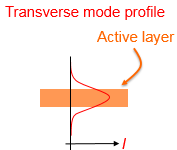
\includegraphics[scale=0.75]{ch5/image45}
	\captionof{figure}{ }
	\end{wrapfigure}
	 Il y a bien évidemment également des contributions de l'émission stimulée ainsi que 
	l'absorption. On le sait, les photons ne sont pas entièrement confiné dans la région 
	active : soit $V_p$ le volume effectif du mode lasant. On peut alors écrire
	\begin{equation}
	{\left(\frac{{{\rm{d}}{n_p}}}{{{\rm{d}}t}}\right)_{sta}} = \frac{V}{{{V_p}}}({R_{st}} - {R_A}) 
	= \Gamma ({R_{st}} - {R_A})
	\end{equation}
	où $V$ est le volume de la zone active et $\Gamma = V/V_p$ est le facteur de confinement 
	(confinement des charges d'un côté et des photons de l'autre). On sait que le taux global 
	d'émission stimulée vaut (résultat obtenu lorsqu'on a établi l'expression du coefficient 
	d'absorption dans les semi-conducteurs).
	\begin{equation}
	({R_{st}} - {R_A}) = {{\cal G}}{v_g}{n_p}
	\end{equation}
	La question est : que vaut $\mathcal{G} = f(n_e)$ ? \\
	
	\begin{wrapfigure}[11]{l}{6cm}
	\vspace{-5mm}
	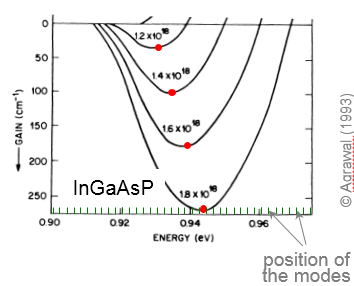
\includegraphics[scale=0.6]{ch5/image46}
	\captionof{figure}{ }
	\end{wrapfigure}	
	Il nous faut un modèle pour le gain. La largeur de celui-ci vaut à peu près 35 meV, quelle
	est la différence d'énergie entre les modes de cavité ? Si on considère un laser FP de longueur
	$L=100\ \mu$ :
	\begin{equation}
	\frac{{\Delta \nu }}{\nu } = \frac{c}{{2L\eta }}\frac{\lambda }{c} = 1.8 \times {10^{ - 3}}\ 
	\to\  \Delta {\rm{E}} = 1.8 \times {10^{ - 3}}{\rm{E}} \approx 1.8{\rm{ meV}}
	\end{equation}
	Il y a donc $\pm10$ modes "en dessous" de la courbe de gain ; il va y avoir lasage à la 
	fréquence\footnote{Pq?}	tel que $\mathcal{G} = \mathcal{G}_\text{max}$. Si l'on plot 
	$\mathcal{G}_\text{max}$ comme	une fonction de $n_e$, on obtient presque une fonction linéaire.\\
	
	\begin{wrapfigure}[10]{r}{5cm}
	\vspace{-5mm}
	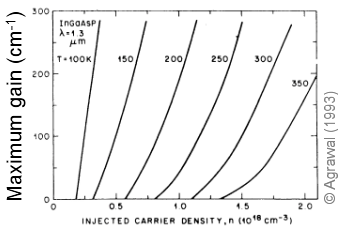
\includegraphics[scale=0.6]{ch5/image47}
	\captionof{figure}{ }
	\end{wrapfigure}	
	Comme on considère ici le modèle le plus simple, ces courbes vont être linéarisée
	\begin{equation}
	{{\cal G}} = {{{\cal G}}_{\max }} \approx a({n_e} - {n_{tr}})
	\end{equation}
	où $a = d\mathcal{G}/dn_e$ est le gain différentiel ($m^2$) et $n_{tr}$ la densité de 
	transparence. Notons que l'augmentation de la température diminue $\mathcal{G}_{\text{max}}$.\\
	
	Il nous reste à modéliser les pertes de photons. Nous avons les pertes internes (absorption, 
	diffusion, défauts, \dots) $\alpha_i$ et les pertes des miroirs ${\alpha _m} =  - \frac{1}{{2L}}
	\ln ({R^2})$.\footnote{Pour un FP : $R = \frac{{{{(n - 1)}^2}}}{{{{(n + 1)}^2}}} \approx 0.3$.}\\
	
	En définissant $a_m = \alpha_i+\alpha_m$, il est possible de définir le temps de vie d'un photon
	dans la cavité
	\begin{equation}
	\frac{1}{{{t_c}}} = {\alpha _c}{v_g} = ({\alpha _i} + {\alpha _m}){v_g}
	\end{equation}
	Ceci nous permet d'exprimer la variation de la densité électronique causée par les pertes
	\begin{equation}
	{\left(\frac{{{\rm{d}}{n_p}}}{{{\rm{d}}t}}\right)_{{\rm{loss}}}} =  - {n_p}/{t_c}
	\end{equation}
	Nous avons ainsi nos deux équations de bilan\\
	
	\cadre{\begin{equation}
	\left\{\begin{array}{lll}
	\DS\frac{{{\rm{d}}{n_e}}}{{{\rm{d}}t}} &\DS= {\eta _i}\frac{{I}}{{qV}} - \frac{{{n_e}}}{\tau
	 } - a({n_e} - {n_{tr}}){v_g}{n_p}&\qquad(1)\vspace{2mm}\\
	\DS\frac{{{\rm{d}}{n_p}}}{{{\rm{d}}t}} &\DS= \Gamma a({n_e} - {n_{tr}}){v_g}{n_p} + {\beta _{sp}}{R_{sp}} - \frac{{{n_p}}}{{{t_c}}}&\qquad(2)
 	\end{array}\right.\qquad\text{ et }\qquad {{\cal G}} = a({n_e} - {n_{tr}})
	\end{equation}}\ \\
	
	\begin{wrapfigure}[6]{r}{4.5cm}
	\vspace{-8mm}
	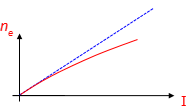
\includegraphics[scale=0.85]{ch5/image48}
	\captionof{figure}{ }
	\end{wrapfigure}		
	Dans le cas stationnaire ${\dot n_e} = {\dot n_p} = 0$. Comme $\beta_{sp} \approx 10^{-4}$, on 
	peut négliger le terme d'émission spontanée. Comme pour les solutions de Maxwell-Bloch, on a 
	deux solutions. La solution triviale est donnée pour $n_p=0$
	\begin{equation}
	{n_e} = {\eta _i}\frac{{I}}{{qV}}\tau 
	\end{equation}
	où $\DS \frac{1}{\tau } = B{n_e} + Cn_e^2$. Le laser est ici en dessous du seuil. On remarque 
	que ce n'est pas totalement linéaire car le temps de vie dépend de la densité électronique (le 
	terme radiatif et le terme de Auger).\\
	
	Regardons maintenant ce qu'il en est pour la solution non-triviale ($n_p\neq 0$). En annulant
	la dérivée temporelle ainsi que le terme en $\beta_{sp}$ dans $(2)$ :
	\begin{equation}
	\underbrace{\frac{{{\rm{d}}{n_p}}}{{{\rm{d}}t}}}_{=0} = \Gamma \underbrace{a({n_e} - {n_{tr}})}_{\mathcal{G}}{v_g}{n_p} + \underbrace{{\beta _{sp}}{R_{sp}}}_{\approx0} - \frac{{{n_p}}}{{{t_c}}}
	\end{equation}
	On retrouve la condition gain = pertes	(condition d'oscillation) :
	\begin{equation}
	\Gamma {{\cal G}}{v_g} = \frac{1}{{{t_c}}}
	\end{equation}
	En explicitant $\mathcal{G}$, on trouve que $\Gamma {{\cal G}} = \Gamma a({n_e} - {n_{tr}}) =
	{\alpha _c}$, cela implique qu'au seul laser nous avons 	 $a({n_{e,th}} - {n_{tr}}) =
	\frac{{{\alpha_c}}}{\Gamma }$, soit encore\\
	
	\cadre{\begin{equation}
	{n_e} = {n_{e,th}} = {n_{tr}} + \frac{{{\alpha _c}}}{{a\Gamma }}
	\end{equation}}\ \\
	
	En divisant par $\tau$
	\begin{equation}
	\frac{{{n_{e,th}}}}{\tau } = {\eta _i}\frac{{I}}{{qV}} - \frac{{{\alpha _c}}}{\Gamma }{v_g}
	{n_p}
	\end{equation}
	En considérant $(1)$ dans le cas stationnaire pour extraire l'expression de la densité 
	électronique au seuil laser 
	\begin{equation}
	{n_p} = \frac{\Gamma }{{{v_g}{\alpha _c}}}({\eta _i}\frac{{I}}{{qV}} - \frac{{{n_{e,th}}}
	}{\tau }) = {\eta _i}\frac{\Gamma }{{{v_g}{\alpha _c}qV}}({I - }{{I}_{th}})
	\end{equation}
	Cette équation met en évidence une variation linéaire de $n_p$ avec $I$. Nous avons ainsi 
	regroupé plusieurs constantes ensemble dans le but de faire apparaître $I-$quelque chose qui
	à les dimensions d'un courant, le seuil laser :
	\begin{equation}
	{{I}_{th}} = {n_{e,th}}\frac{{qV}}{{{\eta _i}}}\frac{1}{\tau }
	\end{equation}
	Ceci nous donne les courbes caractéristiques d'une diode laser
	\begin{center}
	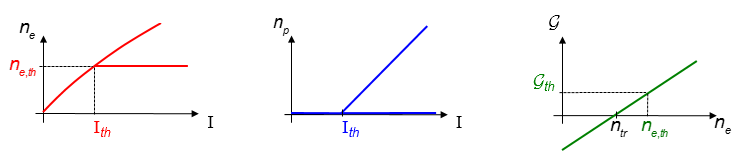
\includegraphics[scale=0.75]{ch5/image49}
	\captionof{figure}{ }
	\end{center}
	On retrouve la variation linéaire de la puissance avec l'intensité. Au delà du seuil il y 
	a deux solutions possibles : une des deux ne serait-elle pas instable? Étudions donc la
	stabilité de la solution triviale
	\begin{equation}
	n_e^{st} = {\eta _i}\frac{{I}}{{qV}}\tau,\qquad n_p=0
	\end{equation}
	Introduisons une petite variation autour de la solution stationnaire
	\begin{equation}
	{n_e} = n_e^{st} + \delta (t),\qquad {n_p} = \varepsilon (t)\quad\text{avec }\ 
	\delta  \ll n_e^{st}\ \ \  {\rm{ et  }}\ \ \ \varepsilon \approx1/{V_p}
	\end{equation}
	Concentrons-nous sur une étude de la stabilité linéaire en linéarisant nos équations 
	différentielles : les termes du second ordres ($\propto \delta\varepsilon$) sont négligés
	\begin{enumerate}
	\item 
	\begin{equation}
	\dot \varepsilon  = \Gamma {v_g}a(n_e^{st} + \delta  - {n_{tr}})\varepsilon  - \frac{\varepsilon }{{{t_c}}}\quad\Rightarrow\quad \varepsilon (t) = \varepsilon (0){{\mathop{\rm e}\nolimits} ^{\lambda t}}
	\end{equation}
	avec $\lambda  = \Gamma {v_g}\overbrace{a(n_e^{st} - {n_{tr}})}^{\mathcal{G}} - t_c^{ - 1}$.
	\item 
	\begin{equation}
	\dot \delta  = {\eta _i}\frac{{I}}{{qV}} - \frac{{n_e^{st}}}{\tau } - \frac{\delta }{\tau } -
	 a(n_e^{st} + \delta  - {n_{tr}}){v_g}\varepsilon 
	\end{equation}
	On en tire
	\begin{equation}
	 \Rightarrow \delta (t) = \delta (0){{\mathop{\rm e}\nolimits} ^{ - t/\tau }} - \frac{{{{\cal G}}{v_g}\varepsilon (0)}}{{\lambda  + 1/\tau }}({{\mathop{\rm e}\nolimits} ^{\lambda t}} - {{\mathop{\rm e}\nolimits} ^{ - t/\tau }})
	\end{equation}
	Il faut que $\lambda < 0$ afin d'avoir une solution stable. En effectuant les calculs (slide 65)
	pour obtenir une expression de $\lambda$, on trouve 
	\begin{equation}
	\lambda  = \frac{{\Gamma {v_g}a}}{{qV}}\tau {\eta _i}({I} - {{I}_{th}})
	\end{equation}
	La solution triviale n'est stable que si $I < I_{th}$.
	\begin{center}
	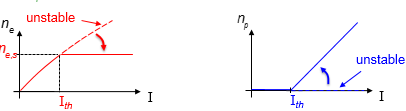
\includegraphics[scale=0.75]{ch5/image50}
	\captionof{figure}{ }
	\end{center}
	\end{enumerate}	
	
	
	\subsection{Puissance laser et rendement}
	Avant toute chose, rappelons le taux de photons perdus	
	\begin{equation}
	{({\dot n_p})_{loss}} =  - {n_p}/{t_c} =  - ({\alpha _i} + {\alpha _m}){v_g}{n_p}
	\end{equation}
	Pour calculer le rendement, il est nécessaire de connaître le taux de photons s'échappant de la
	cavité par unité de volume : $\alpha_mv_gn_p$. Pour exprimer la puissance, il faut tenir compte
	du volume de la cavité. En dessous du seuil laser
	\begin{equation}
	{P_{{\rm{laser}}}} = {\alpha _m}{v_g}{n_p}\hbar {\omega _L}{V_p}
	\end{equation}
	La puissance est en effet le produit entre $\alpha_mv_gn_p$, l'énergie d'un photon et le volume 
	occupé par ces photons dans le laser en question. En exprimant $n_p$
	\begin{equation}
	{P_{{\rm{laser}}}} = {\alpha _m}{v_g}\hbar {\omega _L}{V_p}{\eta _i}\frac{\Gamma }{{{v_g}{\alpha
	 _c}qV}}({I - }{{I}_{th}})
	\end{equation}
	où $\Gamma = V/V_p$. Après simplifications
	\begin{equation}
	{P_{{\rm{laser}}}} = \underbrace{{\eta _i}\frac{{{\alpha _m}}}{{{\alpha _i} + {\alpha _m}}}}
	_{\eta_d}\frac{{\hbar	 {\omega _L}}}{q}({I - }{{I}_{th}})
	\end{equation}
	où $\eta_d$  est le rendement différentiel quantique, soit $\eta_d=\frac{{\Delta {\rm{ number of
	photons out}}}}{{\Delta {\rm{ number of electrons in}}}}$.\\

	\begin{wrapfigure}[6]{r}{4.5cm}
	\vspace{-8mm}
	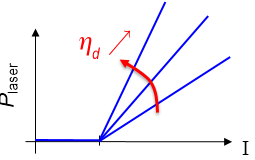
\includegraphics[scale=0.8]{ch5/image51}
	\captionof{figure}{ }
	\end{wrapfigure}			
	Ce coefficient fait le lien entre 
	la recombinaison d'une paire et les photons, $I$ est le terme de pompage dans les lasers à SC.	
	Ce rendement est proportionnel à la pente de la courbe caractéristique $P_{\text{laser}} - I$ : 
	puissance nulle en dessous d'un certain seuil et linéaire au dessus. Forcément, plus la pente 
	est forte, plus le rendement est bon. Le rendement $\eta_d$ augmente (de façon logique) lorsque 
	$\alpha_i$ diminue : il faut minimiser les pertes par diffusion et (ré-)absorption\footnote{On 
	utilisera alors des cristaux avec de faibles densité de défauts (faible absorption et diffusion) 
	ainsi qu'une double héréro-jonction et un guidage d'onde.}.\\
	
	On peut également définir le rendement externe
	\begin{equation}
	{\eta _{ext}} = \frac{{{\rm{number of photons out}}}}{{{\rm{number of electrons in}}}} =
	\frac{{{P_{laser}}/\hbar {\omega _L}}}{{{I}/q}} = {\eta _i}\frac{{{\alpha _m}}}{{{\alpha _i}
	+ {\alpha _m}}}(1{ - }{{I}_{th}}/{I})
	\end{equation}
	Dans le cas limite
	\begin{equation}
	{\eta _{ext}} \to {\rm{ }}{\eta _i}\frac{{{\alpha _m}}}{{{\alpha _i} + {\alpha _m}}}{\rm{  for   
	 }}{I} \gg {{I}_{th}}
	\end{equation}
	On comprend alors l'intérêt de minimiser $I_{th}$. Le slide 67 compare ce résultat à l'expérience
	(vu au cours? Pas de notes).\\
	
	Les performances se dégradent avec la température. Lorsque la température augmente, le 
	gain différentiel($a$) diminue et la densité de transparence ($n_{tr}$) augmente. Il y a 
	également une augmentation des phonons à cause des recombinaisons Auger et, forcément, une 
	diminution de $\eta_i$ par fuite à travers les barrières de potentiels (l'énergie thermique 
	donne l'énergie nécessaire pour sauter la barrière de potentiel)(ci-dessous, à droite). 
	Tout ceci illustre l'importance du contrôle de la température de la diode laser.
	\begin{center}
	\includegraphics[scale=0.6]{ch5/image52}
	\captionof{figure}{ }
	\end{center}
	
\newpage
	\subsection{Propriétés spectrales des diodes lasers}	
	\begin{wrapfigure}[14]{r}{4.5cm}
	\vspace{-5mm}
	\includegraphics[scale=0.7]{ch5/image53}
	\captionof{figure}{ }
	\end{wrapfigure}		
	Ci-contre, le spectre d'un laser à SC en fonction de l'intensité du courant (en certains points).
	Celui-ci est quasi mono-mode, mais il y a quand même une légère pollution venant des autres modes. \\

	Si une face est clivée, cela introduit beaucoup de pertes. En reportant les pertes graphiquement 
	($\alpha_m+\alpha_i$ sont les pertes totales) on peut voir une intersection de la courbe de gain
	avec cette ligne pointillée des pertes totales : il y a lasage à ce mode. Cependant, comme le gain
	est assez important pour d'autres modes adjacent (bien que trop faible pour laser, le gain ne 
	peut plus augmenter car il est saturé à gain = pertes) donnant lieu à un effet de super-radiance. 
	Ils rencontrent un gain assez important qui amplifie à chaque passage, mais pas suffisamment grand 
	que pour compenser les pertes? Les pics satellites ne disparaissent ainsi pas, ils sont juste 
	bloqué et sont petits (étant "super-radiant") par rapport à l'émission laser.
	\begin{center}
	\includegraphics[scale=0.8]{ch5/image54}
	\captionof{figure}{ }
	\end{center}
	Revenons-en à cette partie de la puissance émise à travers modes adjacents. Remarquons tout 
	d'abord que l'ordre des pertes internes, de miroirs et le gain ne changent pas beaucoup aux 
	modes proches
	\begin{equation}
	\alpha_i\approx 40\ cm^{-1},\qquad\qquad \alpha_m\approx 45\ cm^{-1}
	\end{equation}

	\begin{wrapfigure}[10]{r}{3.5cm}
	\vspace{-7mm}
	\includegraphics[scale=0.7]{ch5/image55}
	\captionof{figure}{ }
	\end{wrapfigure}
	Il y a bien donc (comme annoncé un peu plus haut) super-radiance des modes adjacents en dessous
	du seuil laser avec la puissance relative entre le mode lasant et les adjacents qui augmente
	lorsque $I$ augmente au delà de $I_{th}$. Comment éviter le déplacement spectral du spectre et 
	des modes adjacents (laser monomode)?\\
			
	Pour éviter le multimode ou la super-radiance, on peut essayer d'avoir une courbe qui présente des
	pertes importantes pour tous les modes sauf un. Cela garanti que l'on lase à ce mode la et que 
	l'on est en présence d'un monomode longitudinal bloqué à une seule valeur.\\
\newpage	
	En pratique on va utilisé un miroir périodique. Il s'agit d'une structure périodique qui réfléchi
	partiellement la lumière pour les longueurs d'onde qui satisfont à la réflexion de Bragg, les 
	autres passent ou sont (plus) faiblement réfléchies. Les \textit{lasers DBR} (Distributed 
	Bragg Reflector laser). En reportant sur un même graphique le gain (rouge) et les pertes (vert, 
	l'inverse de la réflectivité (réflectivité maximale = pertes minimales)) on aura bien 
	réflexion laser pour un mode et ce même si on shift un peu\footnote{Laser DFB à expliciter, je 
	n'ai pas bien compris}.
	\begin{center}
	\includegraphics[scale=0.6]{ch5/image56}
	\captionof{figure}{ }
	\end{center}